\documentclass{beamer}
\usepackage[utf8]{inputenc}
\usepackage{siunitx}
\usepackage{amsmath}
\usepackage{slashed}
\usepackage{adjustbox}
\usepackage{xcolor}
\hypersetup{
    colorlinks=true,
    linkcolor=blue,
    filecolor=magenta,      
    urlcolor=cyan,
}
\usepackage{hyperref}
\usepackage{multicol}
%#\usepackage{multirow}
\usetheme{boxes}
\newcommand{\Ks}{\ensuremath{K_S^0}}
\newcommand{\ks}{\ensuremath{K_S^0}}
\newcommand{\dd}{\ensuremath{\Delta \delta_D}}
\newcommand{\kspipi}{\ensuremath{\ks \pi^+ \pi^-}}
\newcommand{\Kspipi}{\ensuremath{\ks \pi^+ \pi^-}}
\newcommand{\diffDtokspipi}{\ensuremath{\kspipi{D^0}} \text{and} \ensuremath{\kspipi{\bar{D}^0}} }
\newcommand{\MP}{\ensuremath{m^2_+}}
\newcommand{\MM}{\ensuremath{m^2_-}}
\newcommand{\MZ}{\ensuremath{m^2_0}}
\newcommand{\psires}{\ensuremath{\psi(3770)}}
\newcommand{\phasePosition}{\ensuremath{m^2_+,m^2_-}}
\newcommand{\phasePositionT}{\ensuremath{m^2_-,m^2_+}}
\newcommand{\Dzbar}{\ensuremath{\bar{D}^0} }
\newcommand{\Dz}{\ensuremath{D^0} }
\newcommand{\Bzbar}{\ensuremath{\bar{B}^0} }
\newcommand{\Bz}{\ensuremath{B^0} }
\newcommand{\z}{\ensuremath{\textbf{z}}}
%These macros are save time, usage
%\subAmp{particle}{component} -e.g \subAmp{\Dz}{L_{\pi^+\pi^-}=0}
\newcommand{\subAmp}[2]{\ensuremath{A_{#1}^{#2}\left(\phasePosition \right)}}
%\modelAmp{particle}{model name} - e.g. \modelAmp{\Dz}{Belle}
\newcommand{\modelAmp}[2]{\ensuremath{A_{#1}^{\text{#2}}\left(\phasePosition \right)}}
\newcommand{\genAmp}[2]{\ensuremath{A_{#1}^{\text{#2}}\left(\mathcal{P} \right)}}
%Generic input amp (actually you could use \modelAmp instead if you want
\newcommand{\inputAmp}[1]{\ensuremath{A_{#1}^{\text{input}}\left(\phasePosition\right)}}
%True model - what the decay really is
\newcommand{\trueAmp}[1]{\ensuremath{A_{#1}^{\text{True}}\left(\phasePosition\right)}}
%a_r and phi_r, again saves writing $, _, ^ everywhere
\newcommand{\magPar}[1]{\ensuremath{a_{#1}}}
\newcommand{\phPar}[1]{\ensuremath{\phi_{#1}}}
\newcommand{\KK}{\ensuremath{K^+ K^-}}
\newcommand{\Kppim}{\ensuremath{K^+ \pi^-}}
\newcommand{\Kmpip}{\ensuremath{K^- \pi^+}}
\newcommand{\Kspiz}{\ensuremath{\ks \pi^0}}
\newcommand{\kspiz}{\ensuremath{\ks \pi^0}}
\title{Progress for the Quasi-Model independent method to extract $\dd$ from correlated $D \to \kspipi$ decays}
\begin{document}
\begin{frame}{}
    \maketitle
\end{frame}
\begin{frame}{Overview}
    \begin{itemize}
        \item Likelihood scan performed for a variety of tags, $\KK, \Kppim, \Kmpip, \Kspiz, \Kspipi$ and the combined likelihood for the ``CP'' polynomial.
        \item The combined likelihood needed to be remade (backup slides + appendix in note). In short there was a bug in the C++ code which made the initial implementation of the combined likelihood crash, this new implementation does not crash. 
        \item The time taken for the scan was longer due to this problem + the length of time to perform the scans.
        \item Some parameters aren't included since the plots aren't shown because the scan crashed.
    \end{itemize}
\end{frame}

\begin{frame}{Likelihood Scan for $C_{00}^{-}$}
\begin{figure}
    \centering
        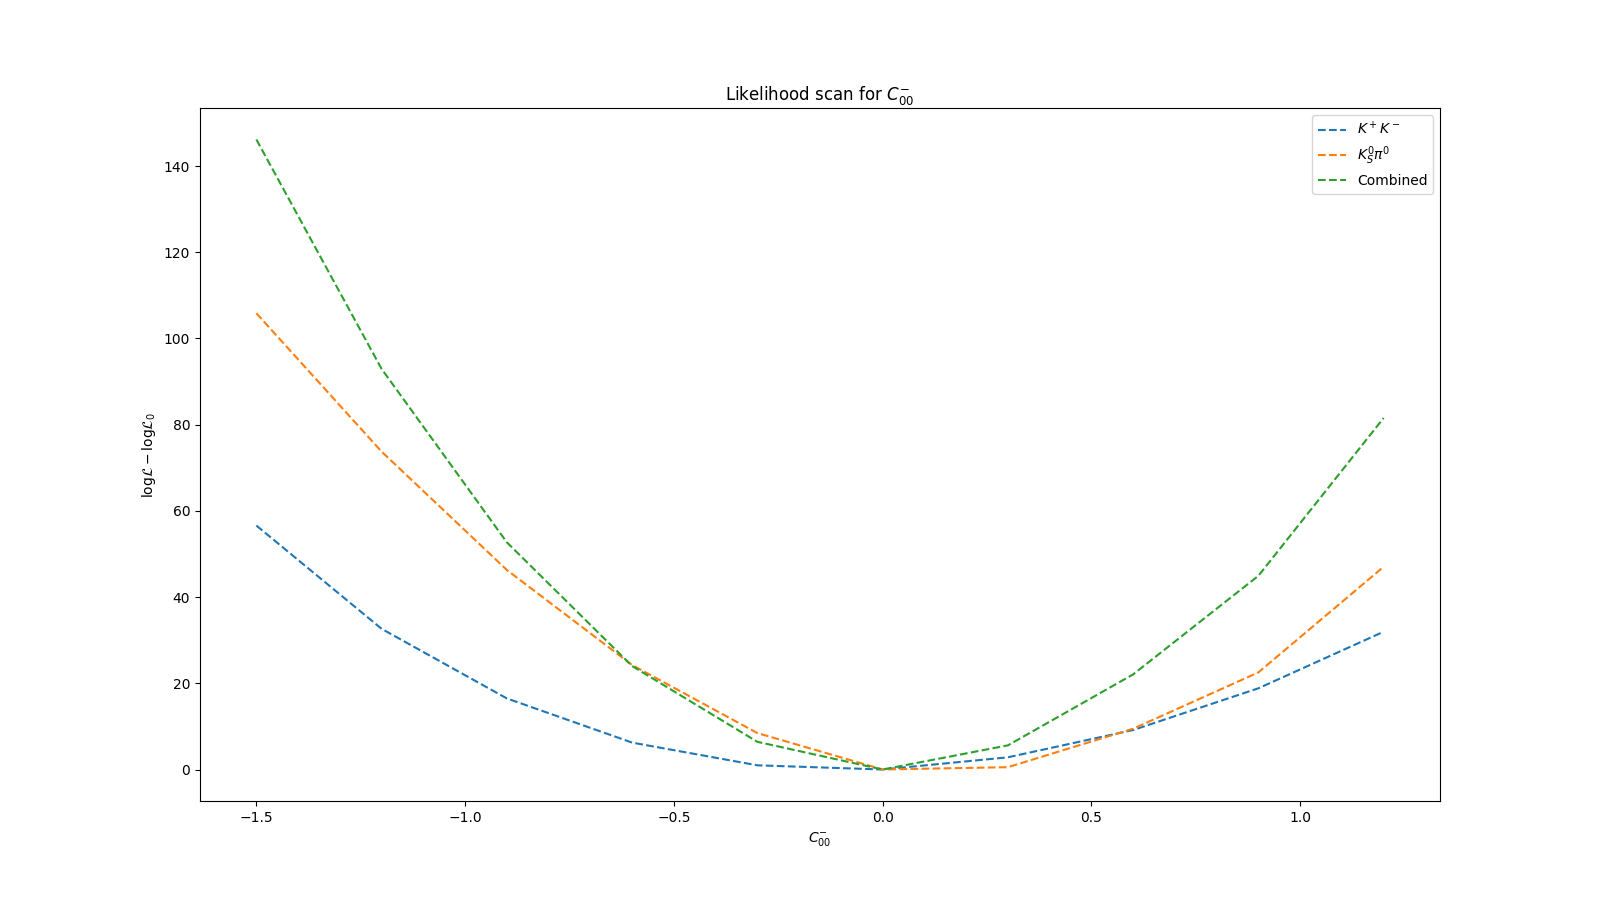
\includegraphics[width=\textwidth]{2020_04_23/figs/M00_Norm.png}
    \caption{Likelihood Scan for $C_{00}^{-}$, where the $y$ axis measures the `distance' of the log likelihood at one value of $C_{10}^{-}$ from the smallest log-likelihood in the sample.}
    \label{fig:scanCM00}
\end{figure}
\end{frame}


\begin{frame}{Likelihood Scan for $C_{01}^{-}$}
\begin{figure}
    \centering
        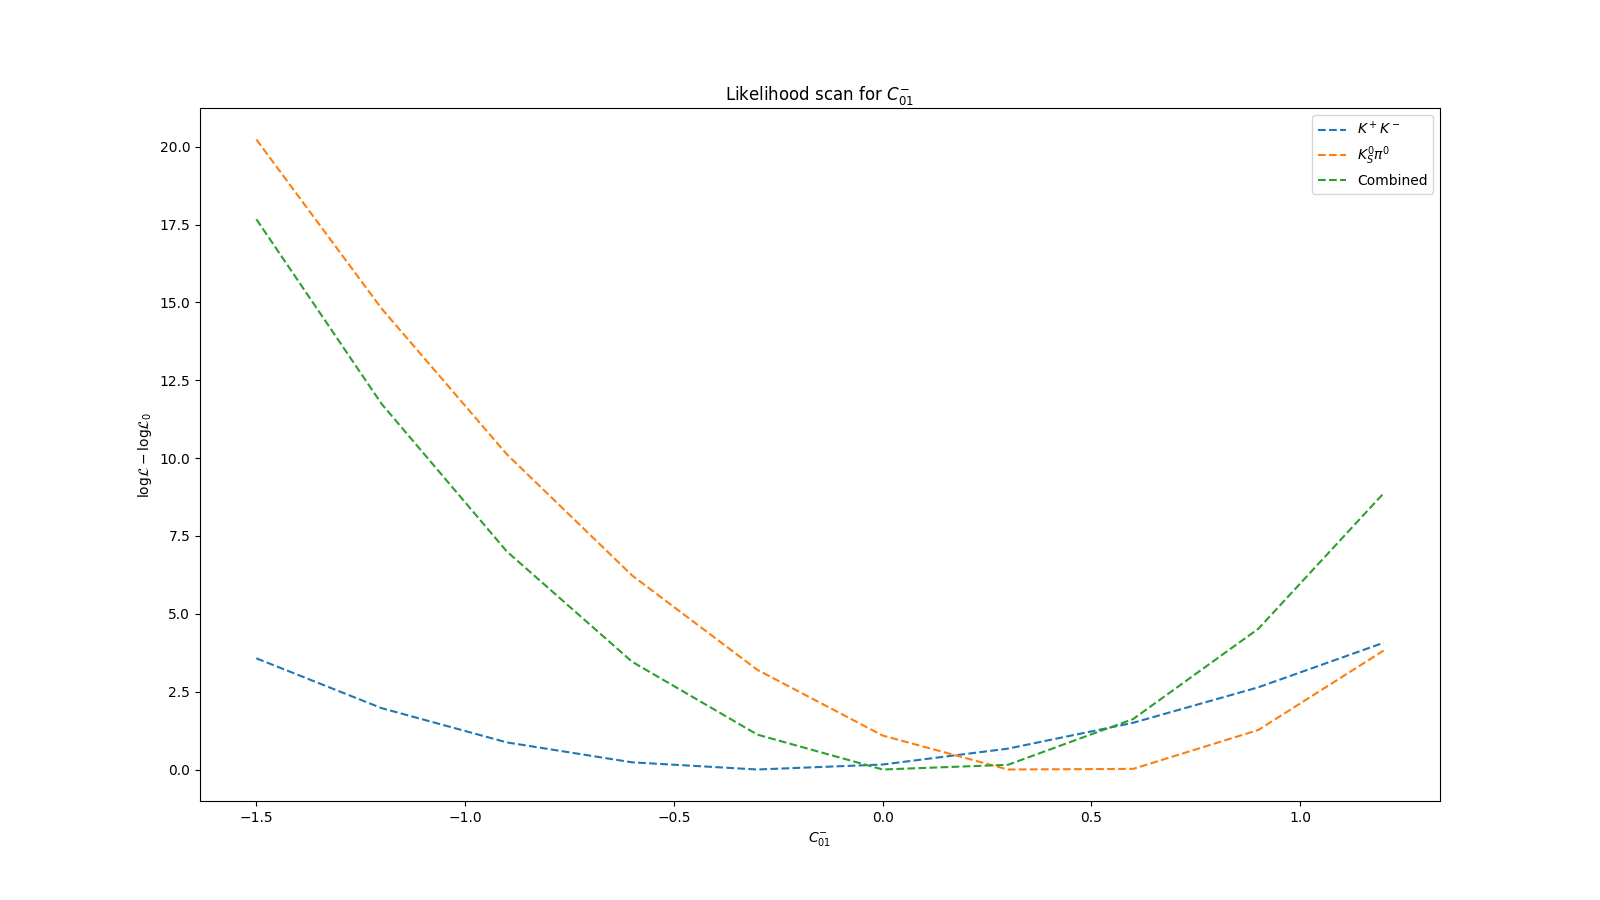
\includegraphics[width=\textwidth]{2020_04_23/figs/M01_Norm.png}
    \caption{Likelihood Scan for $C_{01}^{-}$, where the $y$ axis measures the `distance' of the log likelihood at one value of $C_{10}^{-}$ from the smallest log-likelihood in the sample.}
    \label{fig:scanCM01}
\end{figure}
\end{frame}

\begin{frame}{Likelihood Scan for $C_{10}^{-}$}
\begin{figure}
    \centering
        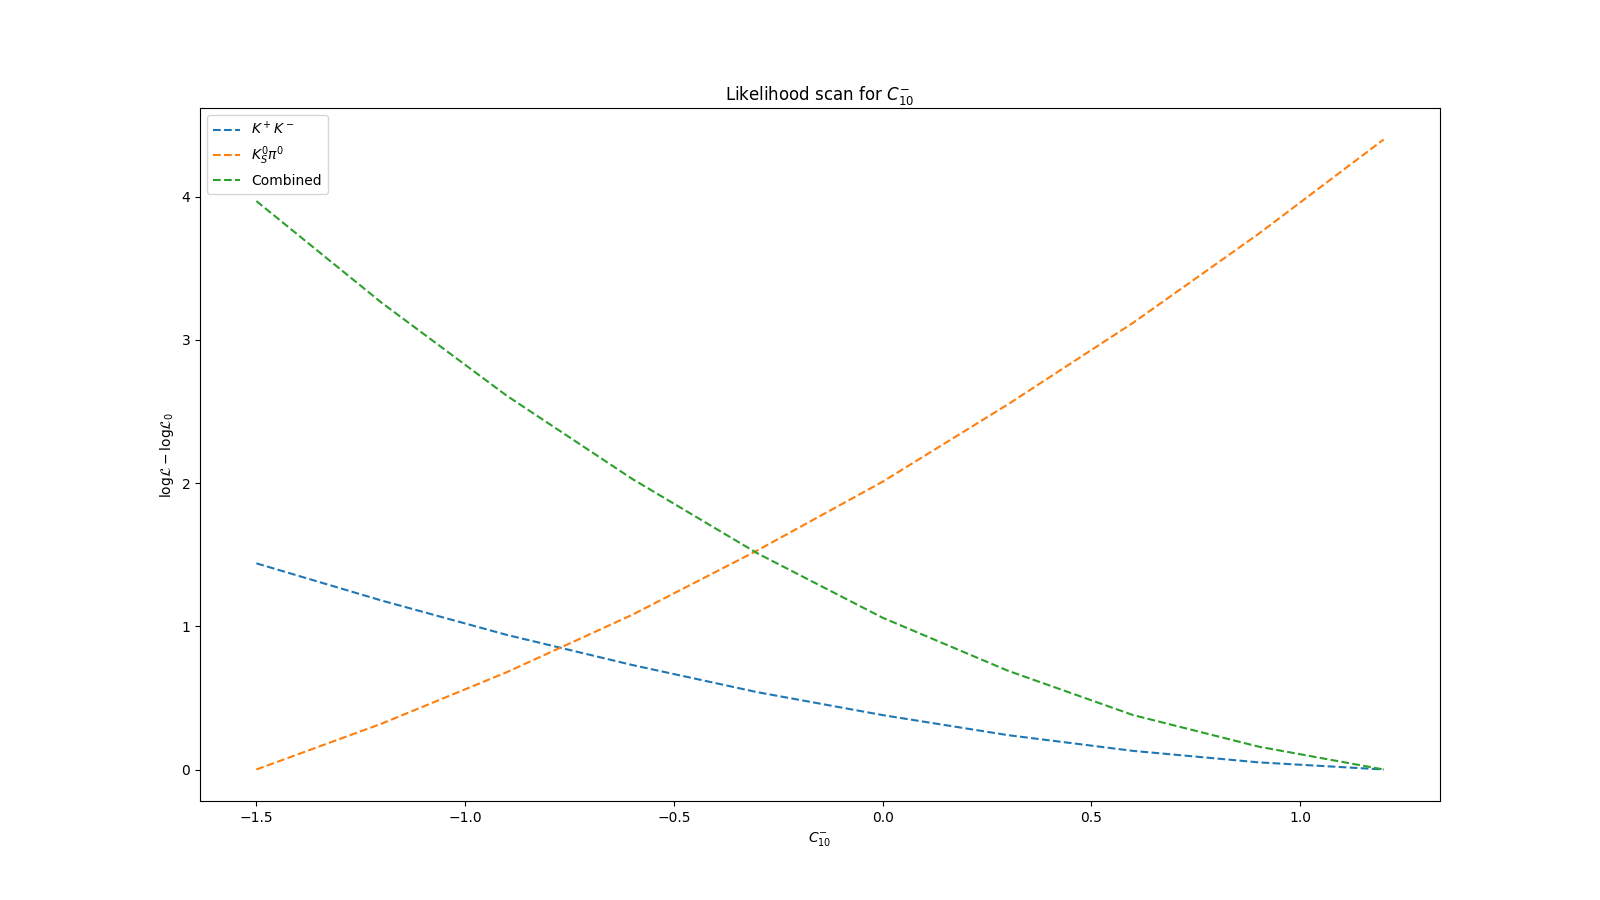
\includegraphics[width=\textwidth]{2020_04_23/figs/M10_Norm.png}
    \caption{Likelihood Scan for $C_{10}^{-}$, where the $y$ axis measures the `distance' of the log likelihood at one value of $C_{10}^{-}$ from the smallest log-likelihood in the sample.}
    \label{fig:scanCM10}
\end{figure}
\end{frame}

\begin{frame}{Likelihood Scan for $C_{02}^{-}$}
\begin{figure}
    \centering
        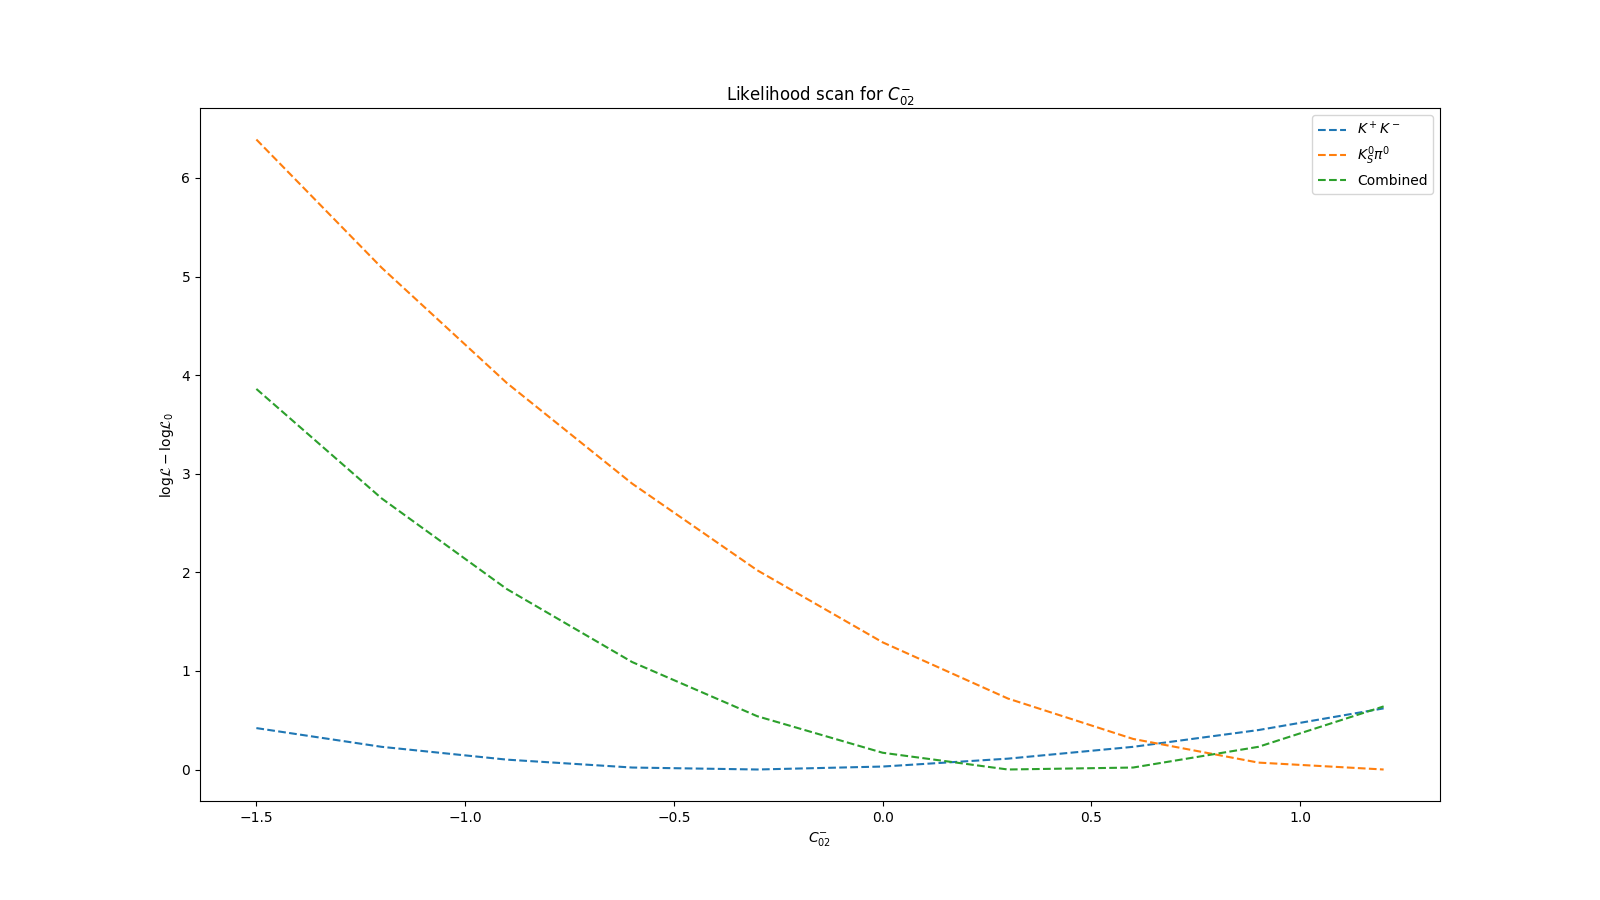
\includegraphics[width=\textwidth]{2020_04_23/figs/M02_Norm.png}
    \caption{Likelihood Scan for $C_{02}^{-}$, where the $y$ axis measures the `distance' of the log likelihood at one value of $C_{10}^{-}$ from the smallest log-likelihood in the sample.}
    \label{fig:scanCM02}
\end{figure}
\end{frame}

\begin{frame}{Likelihood Scan for $C_{11}^{-}$}
\begin{figure}
    \centering
        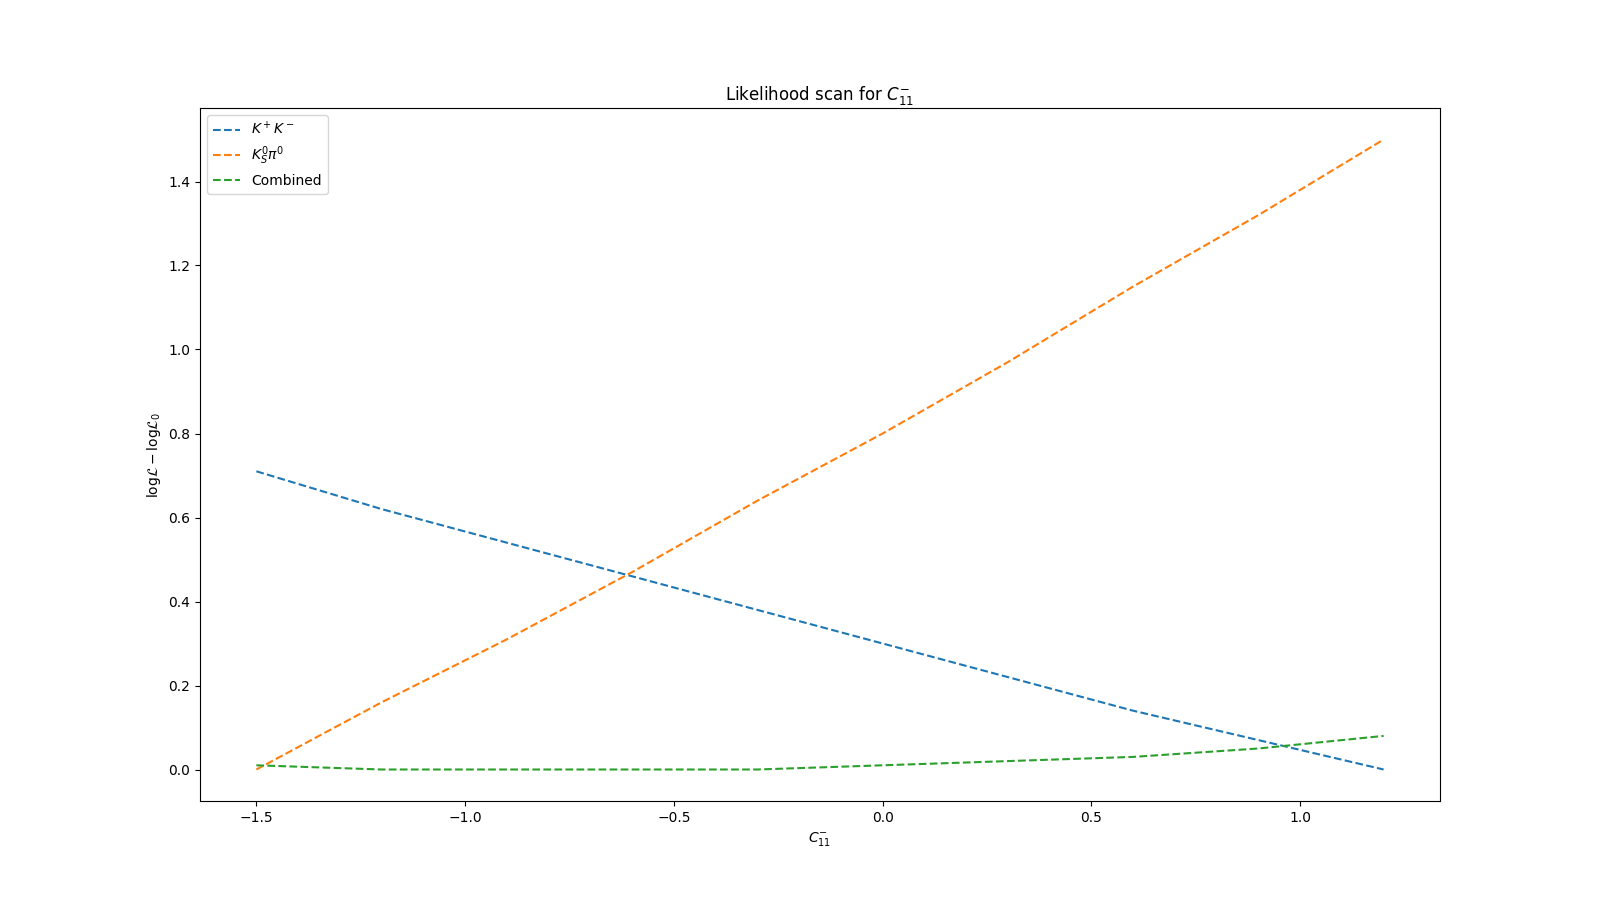
\includegraphics[width=\textwidth]{2020_04_23/figs/M11_Norm.png}
    \caption{Likelihood Scan for $C_{11}^{-}$, where the $y$ axis measures the `distance' of the log likelihood at one value of $C_{10}^{-}$ from the smallest log-likelihood in the sample.}
    \label{fig:scanCM11}
\end{figure}
\end{frame}


\begin{frame}{Likelihood Scan for $C_{20}^{-}$}
\begin{figure}
    \centering
        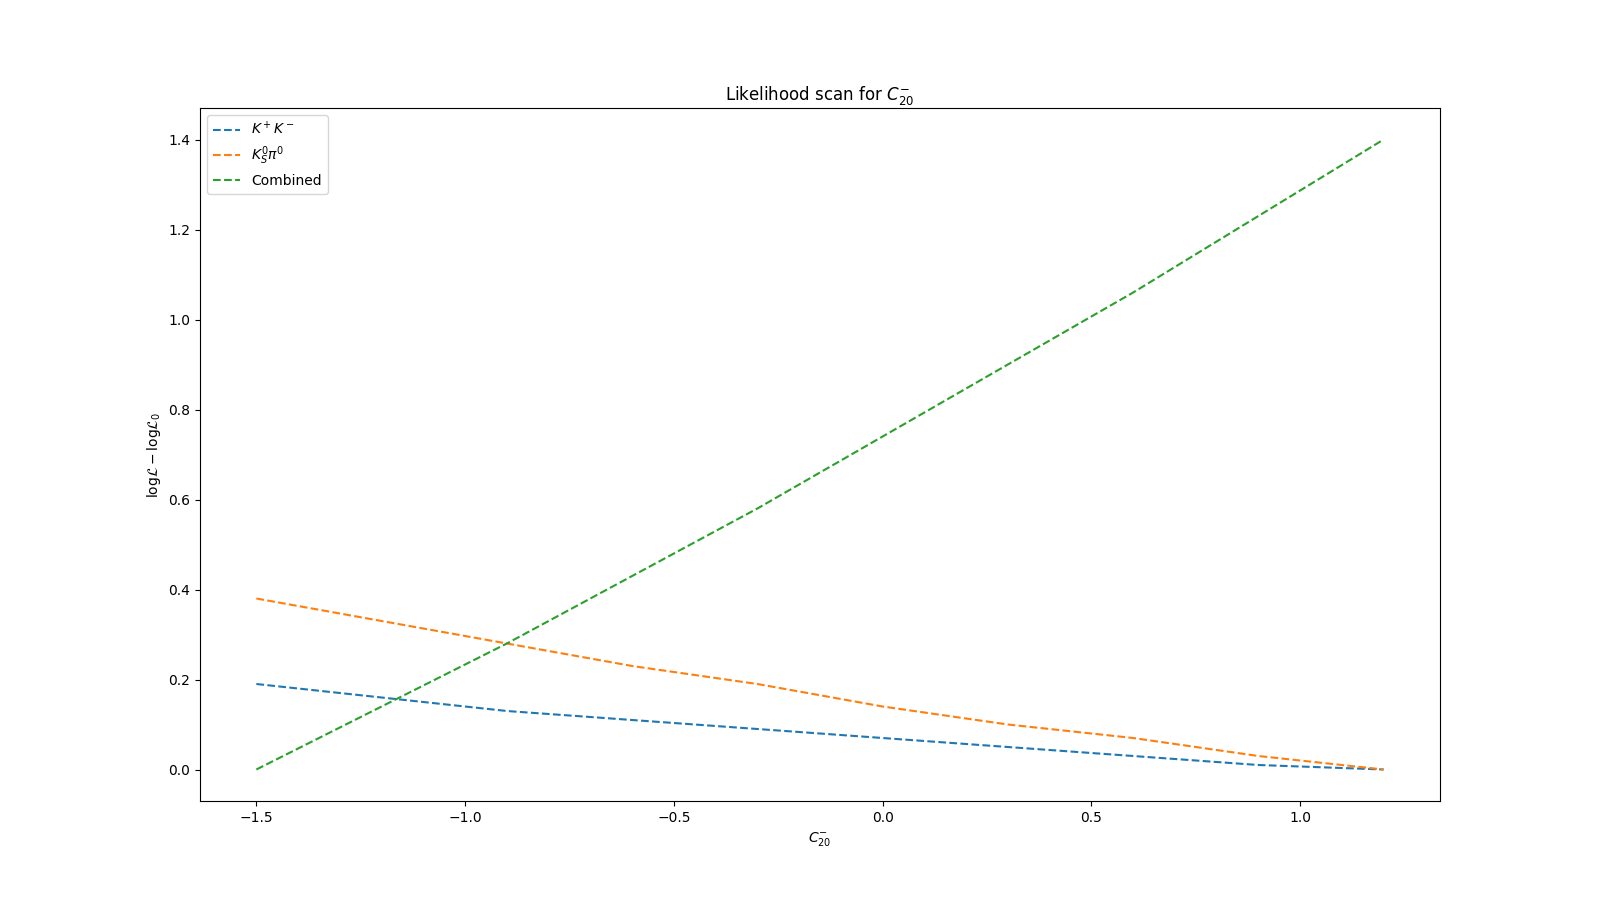
\includegraphics[width=\textwidth]{2020_04_23/figs/M20_Norm.png}
    \caption{Likelihood Scan for $C_{20}^{-}$, where the $y$ axis measures the `distance' of the log likelihood at one value of $C_{10}^{-}$ from the smallest log-likelihood in the sample.}
    \label{fig:scanCM20}
\end{figure}
\end{frame}





\begin{frame}{Likelihood Scan for $C_{00}^{+}$}
\begin{figure}
    \centering
        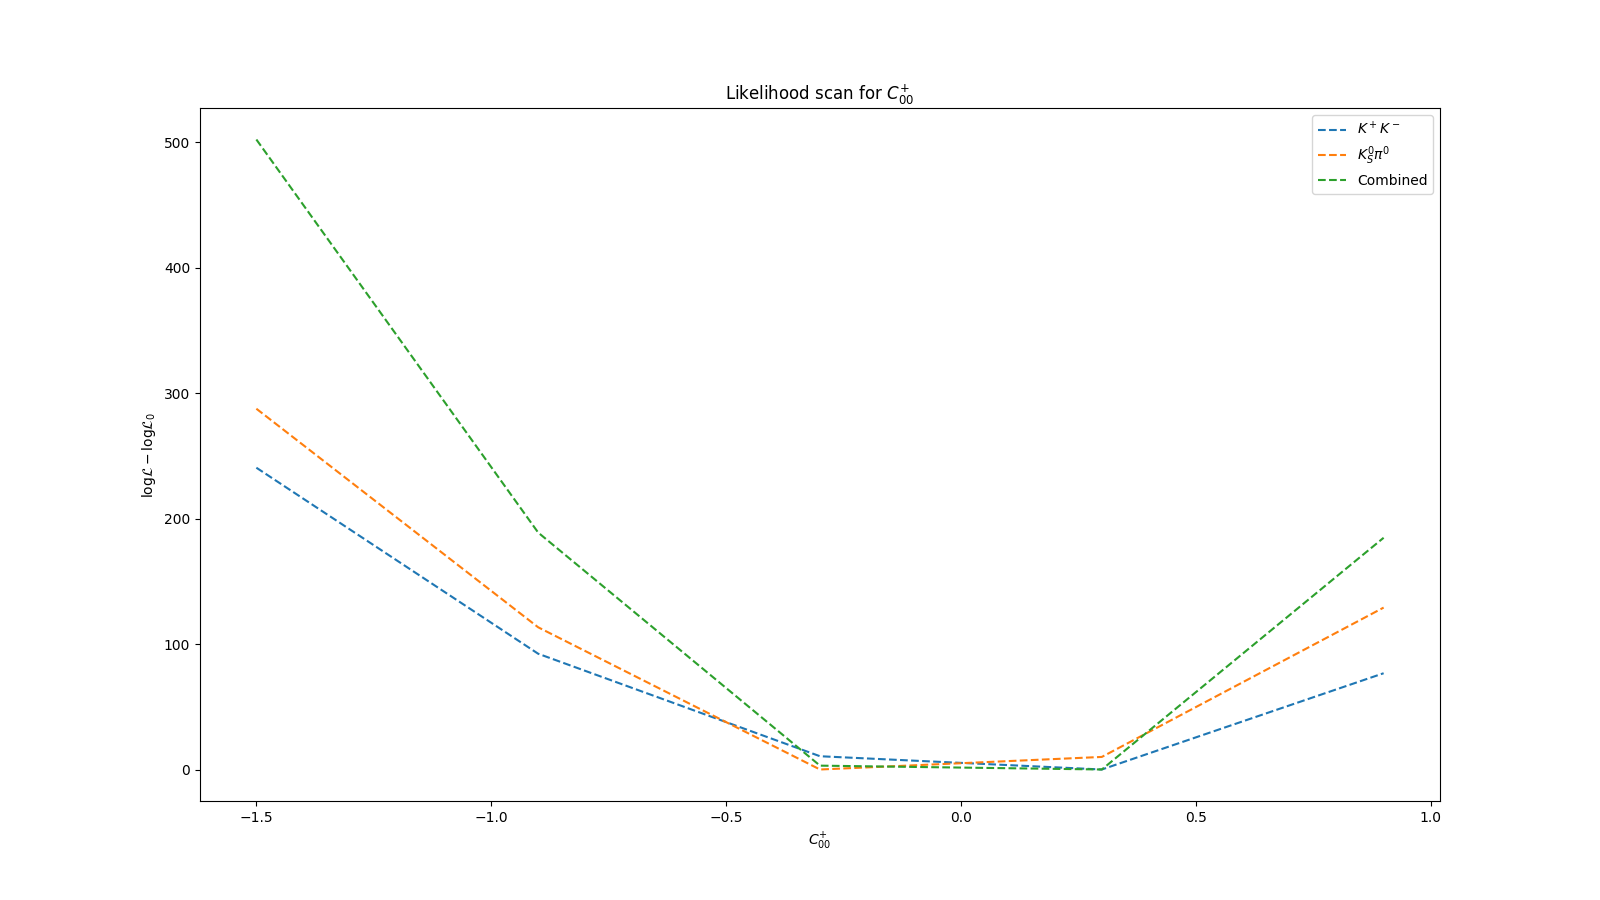
\includegraphics[width=\textwidth]{2020_04_23/figs/P00_Norm.png}
    \caption{Likelihood Scan for $C_{00}^{+}$, where the $y$ axis measures the `distance' of the log likelihood at one value of $C_{00}^{+}$ from the smallest log-likelihood in the sample.}
    \label{fig:scanCP01}
\end{figure}
\end{frame}

\begin{frame}{Likelihood Scan for $C_{01}^{+}$}
\begin{figure}
    \centering
        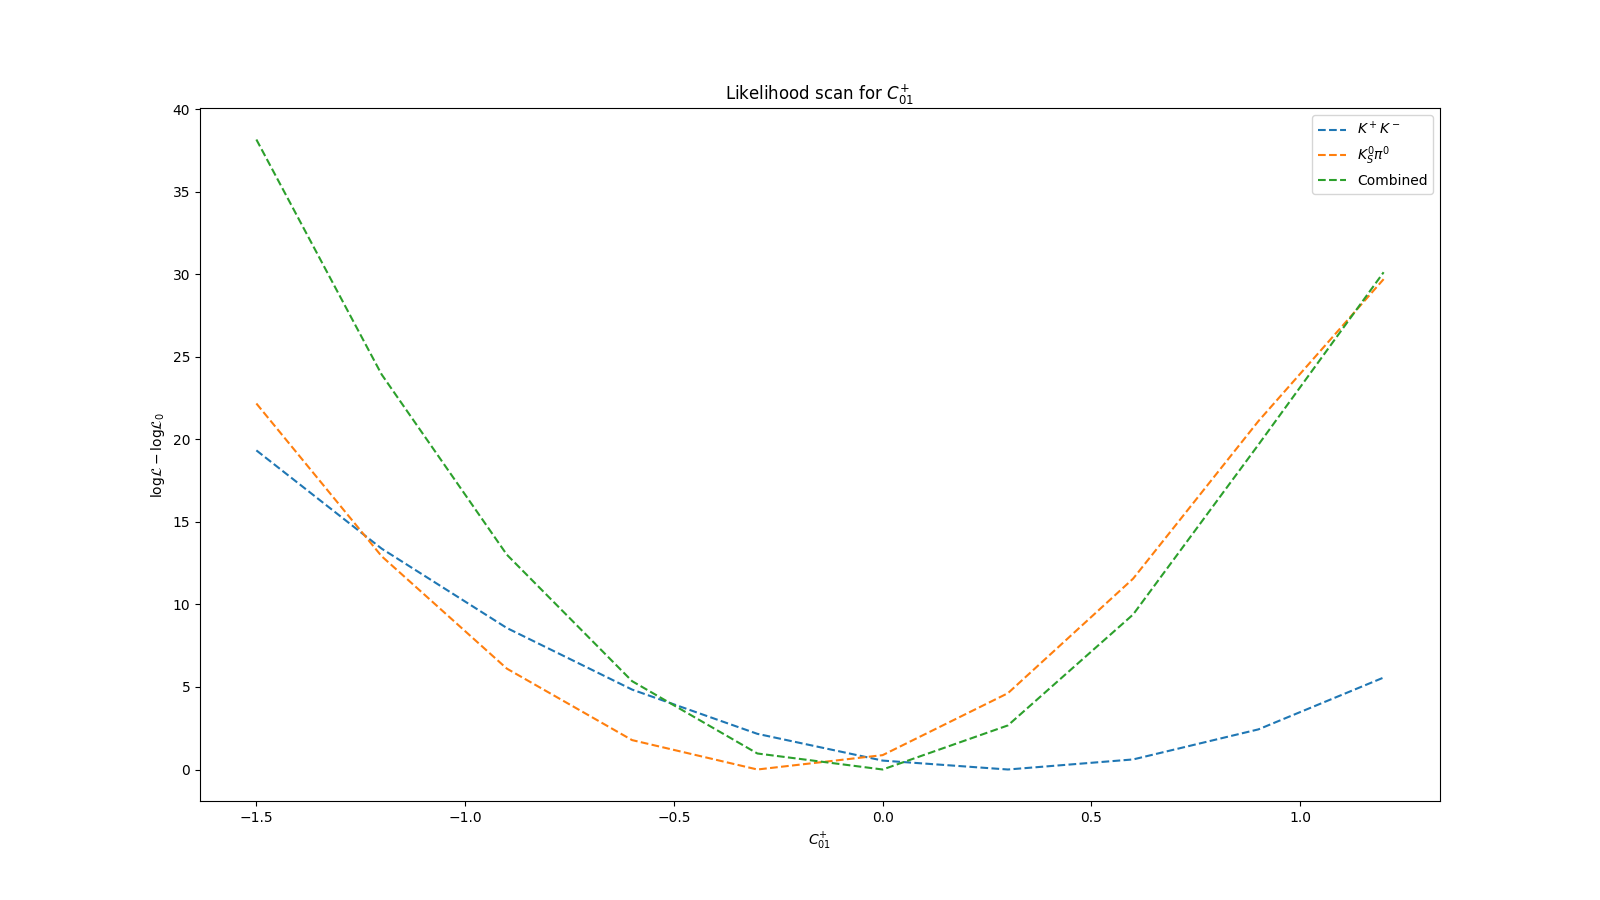
\includegraphics[width=\textwidth]{2020_04_23/figs/P01_Norm.png}
    \caption{Likelihood Scan for $C_{01}^{+}$, where the $y$ axis measures the `distance' of the log likelihood at one value of $C_{10}^{+}$ from the smallest log-likelihood in the sample.}
    \label{fig:scanCP01}
\end{figure}
\end{frame}

\begin{frame}{Likelihood Scan for $C_{10}^{+}$}
\begin{figure}
    \centering
        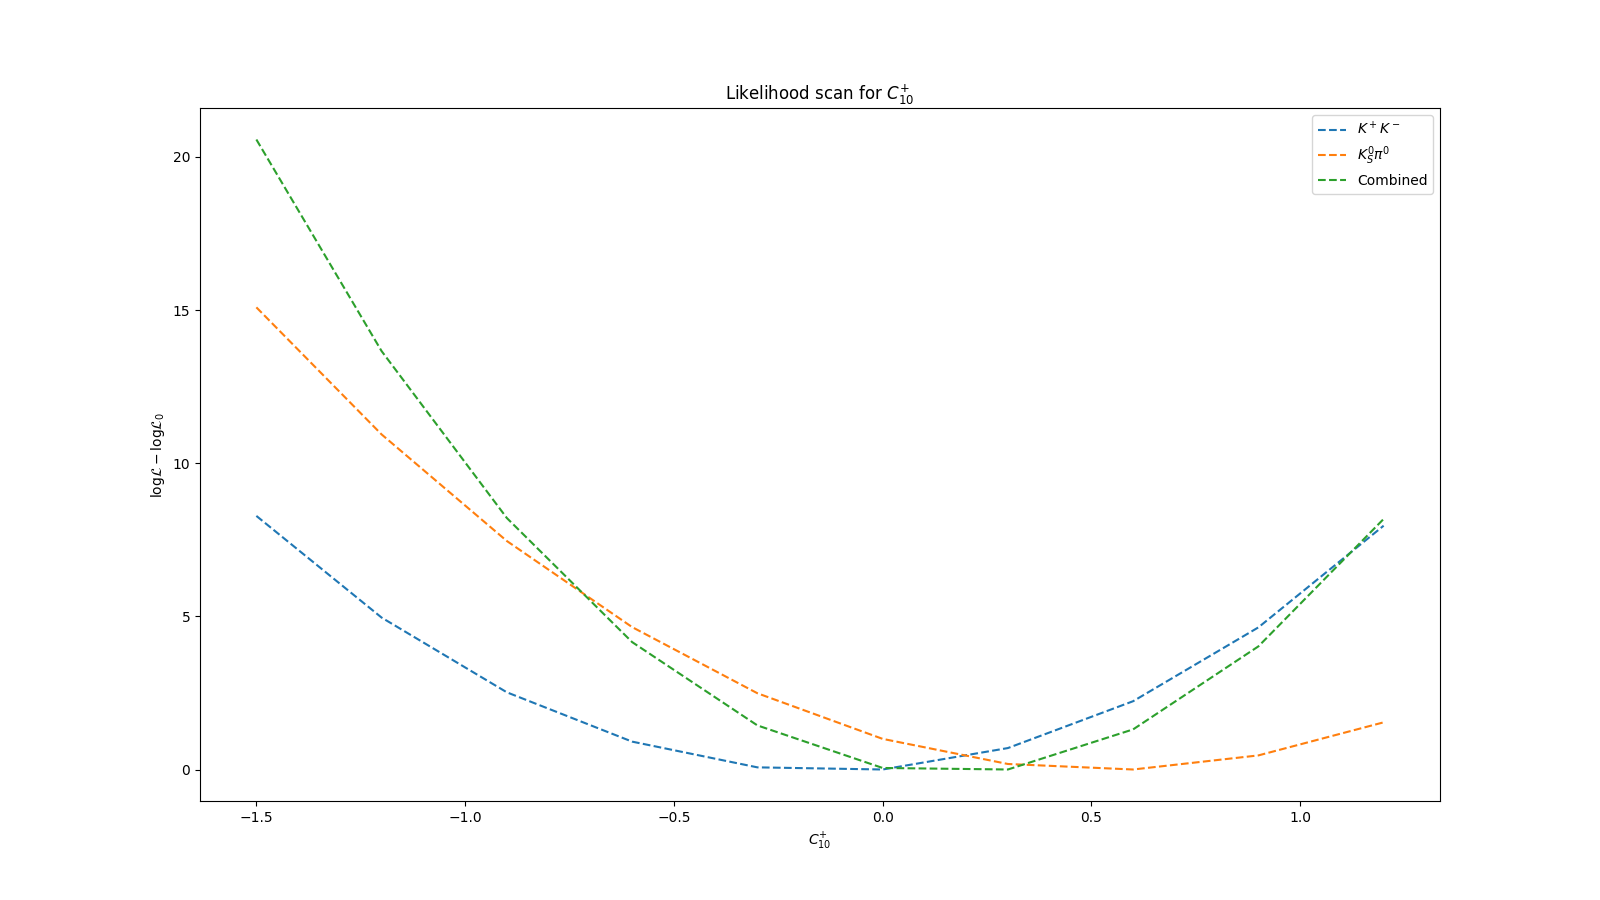
\includegraphics[width=\textwidth]{2020_04_23/figs/P10_Norm.png}
    \caption{Likelihood Scan for $C_{10}^{+}$, where the $y$ axis measures the `distance' of the log likelihood at one value of $C_{10}^{+}$ from the smallest log-likelihood in the sample.}
    \label{fig:scanCP10}
\end{figure}
\end{frame}

\begin{frame}{Likelihood Scan for $C_{02}^{+}$}
\begin{figure}
    \centering
        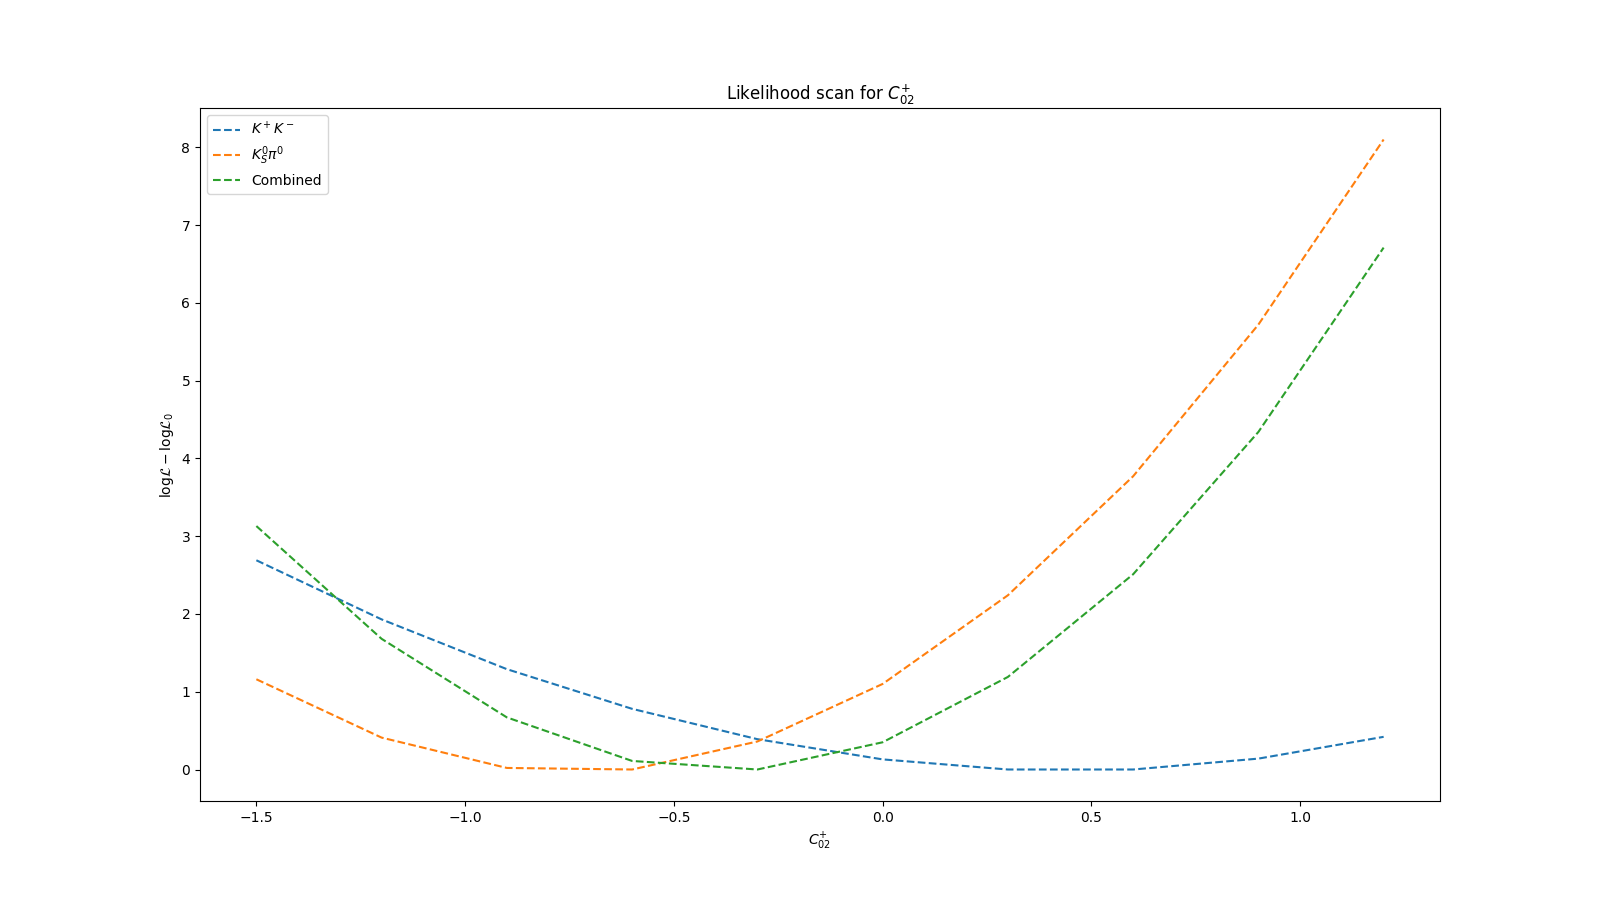
\includegraphics[width=\textwidth]{2020_04_23/figs/P02_Norm.png}
    \caption{Likelihood Scan for $C_{02}^{+}$, where the $y$ axis measures the `distance' of the log likelihood at one value of $C_{02}^{+}$ from the smallest log-likelihood in the sample.}
    \label{fig:scanCP02}
\end{figure}
\end{frame}

\begin{frame}{Likelihood Scan for $C_{11}^{+}$}
\begin{figure}
    \centering
        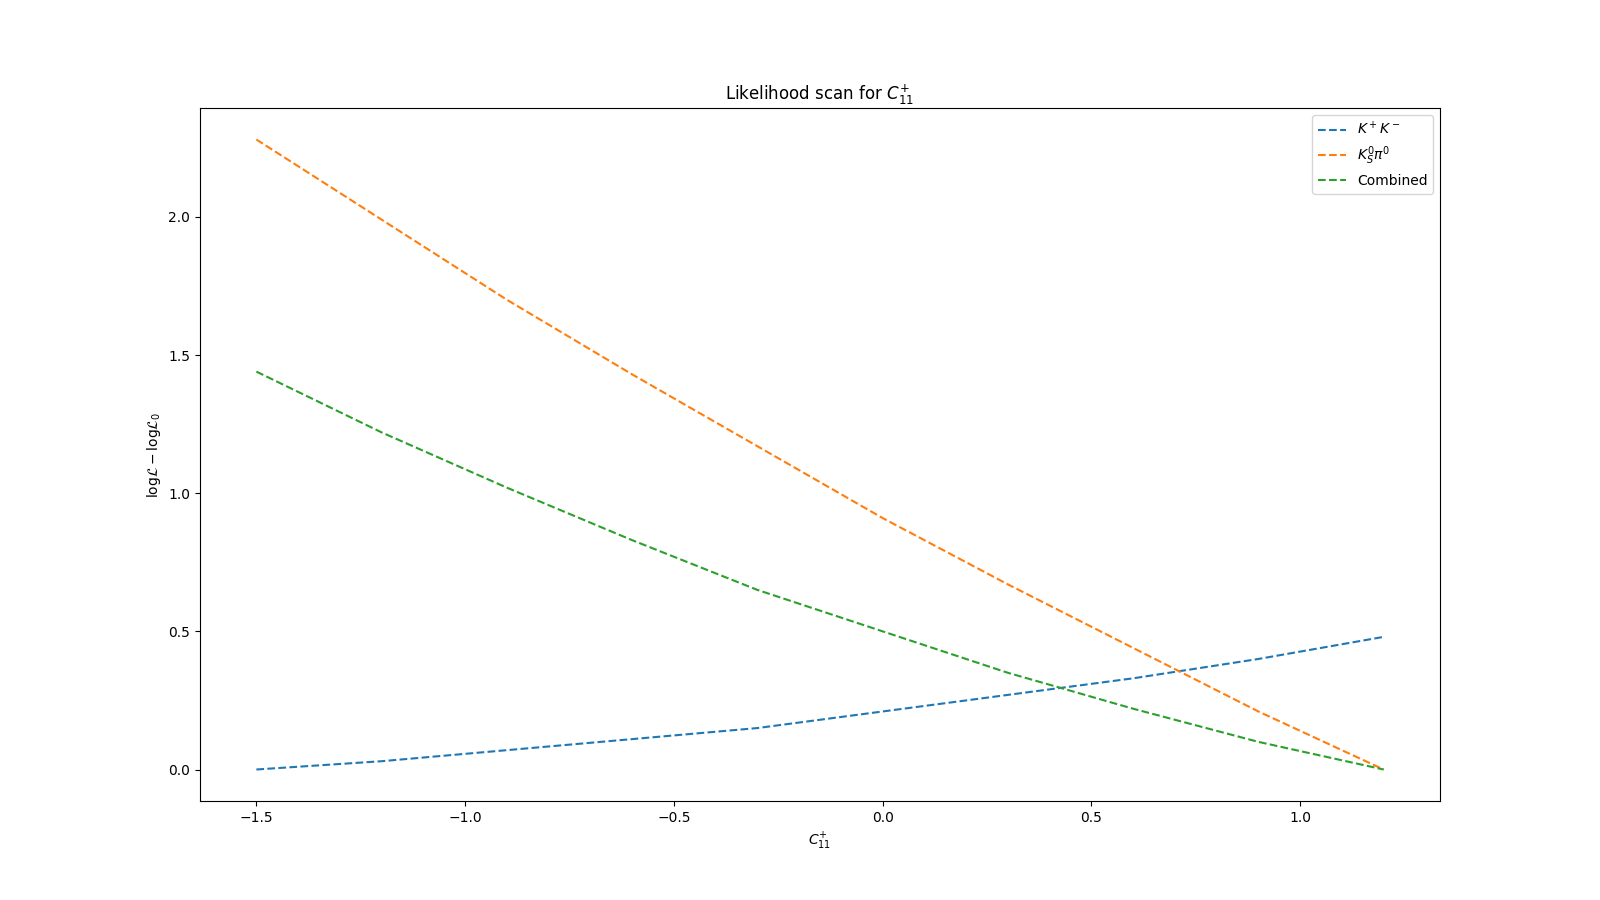
\includegraphics[width=\textwidth]{2020_04_23/figs/P11_Norm.png}
    \caption{Likelihood Scan for $C_{11}^{+}$, where the $y$ axis measures the `distance' of the log likelihood at one value of $C_{11}^{+}$ from the smallest log-likelihood in the sample.}
    \label{fig:scanCP11}
\end{figure}
\end{frame}


\begin{frame}{Likelihood Scan for $C_{20}^{+}$}
\begin{figure}
    \centering
        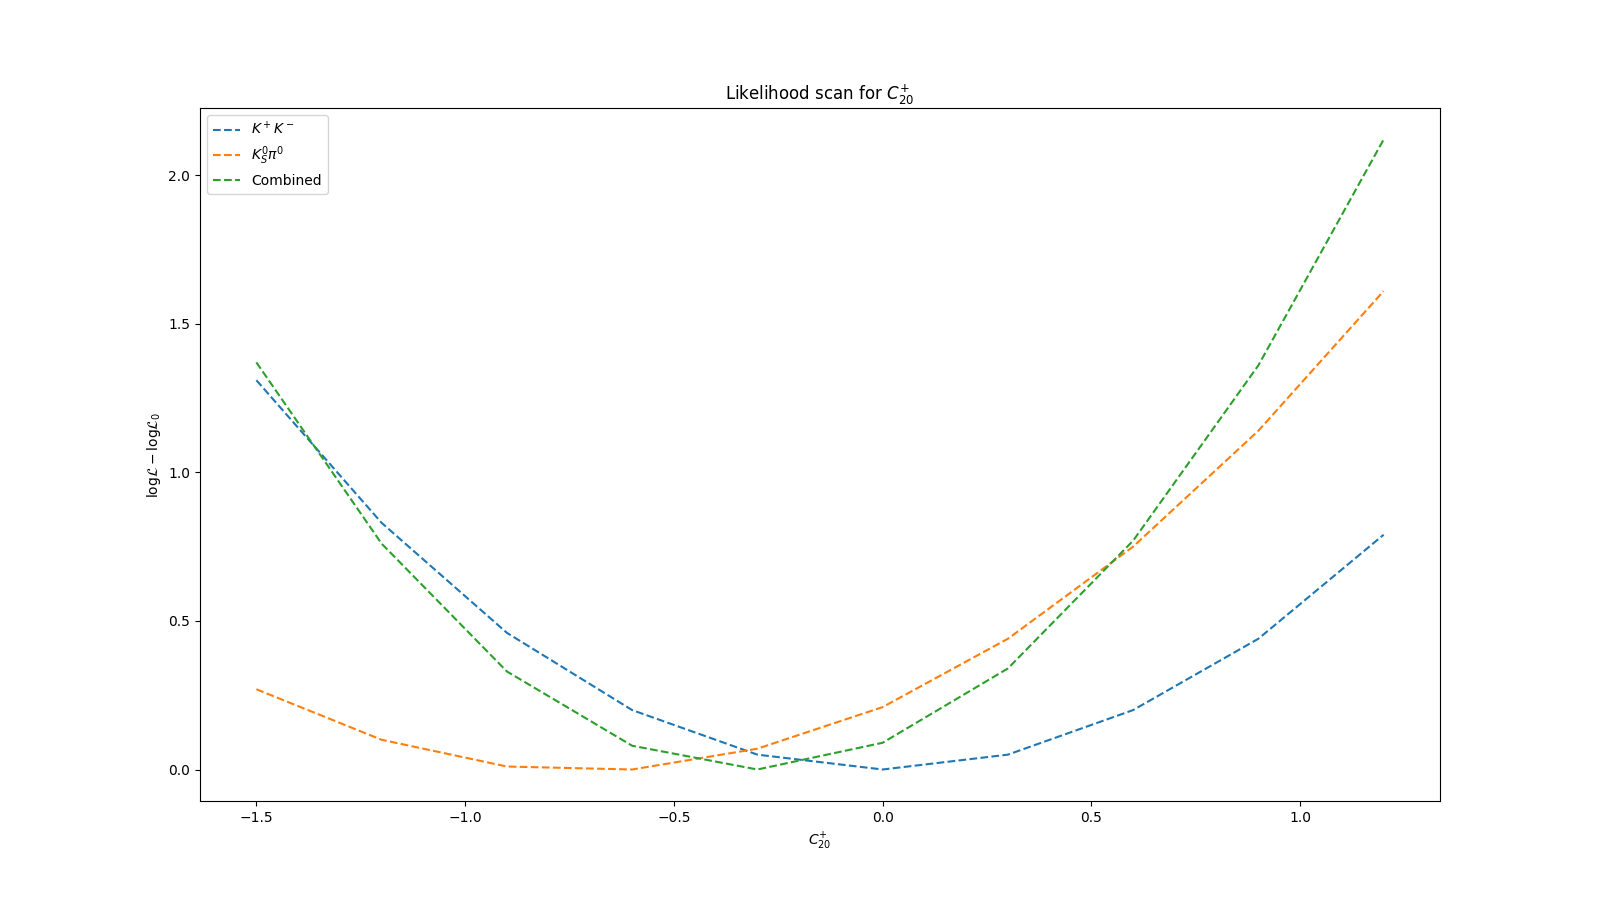
\includegraphics[width=\textwidth]{2020_04_23/figs/P20_Norm.png}
    \caption{Likelihood Scan for $C_{20}^{+}$, where the $y$ axis measures the `distance' of the log likelihood at one value of $C_{20}^{+}$ from the smallest log-likelihood in the sample.}
    \label{fig:scanCP20}
\end{figure}
\end{frame}

\begin{frame}
Backup Slides
\end{frame}

\begin{frame}{Likelihood Scan for $C_{00}^{-}$}
\begin{figure}
    \centering
        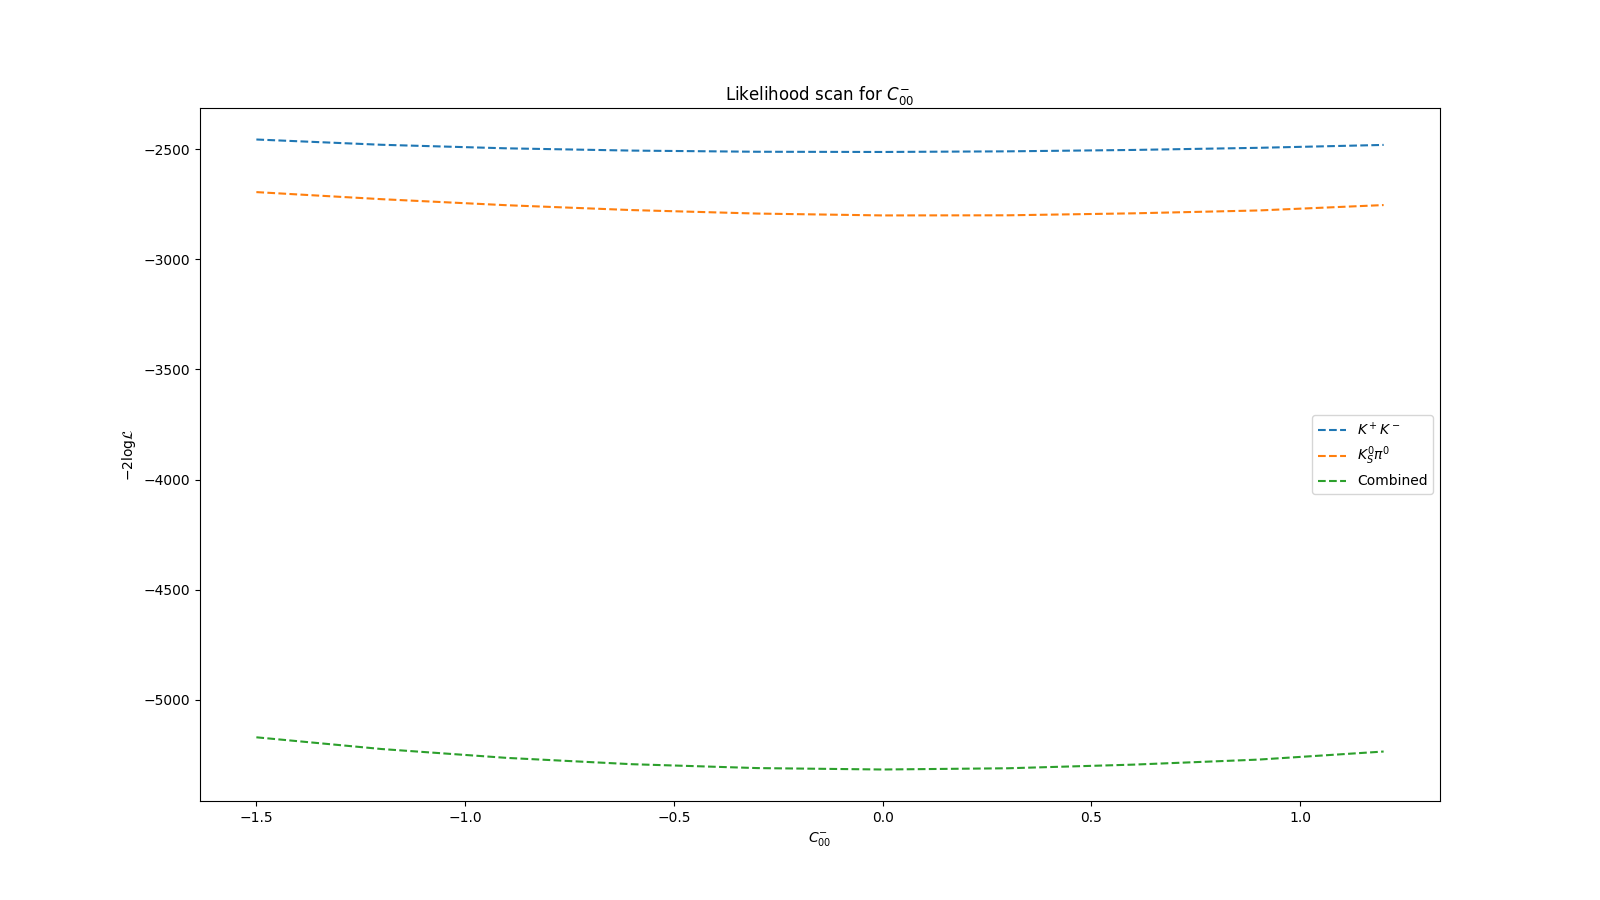
\includegraphics[width=\textwidth]{2020_04_23/figs/M00.png}
    \caption{Likelihood Scan for $C_{00}^{-}$, where the $y$ axis measures the `distance' of the log likelihood at one value of $C_{00}^{-}$.}
    \label{fig:scanCM01}
\end{figure}
\end{frame}

\begin{frame}{Likelihood Scan for $C_{01}^{-}$}
\begin{figure}
    \centering
        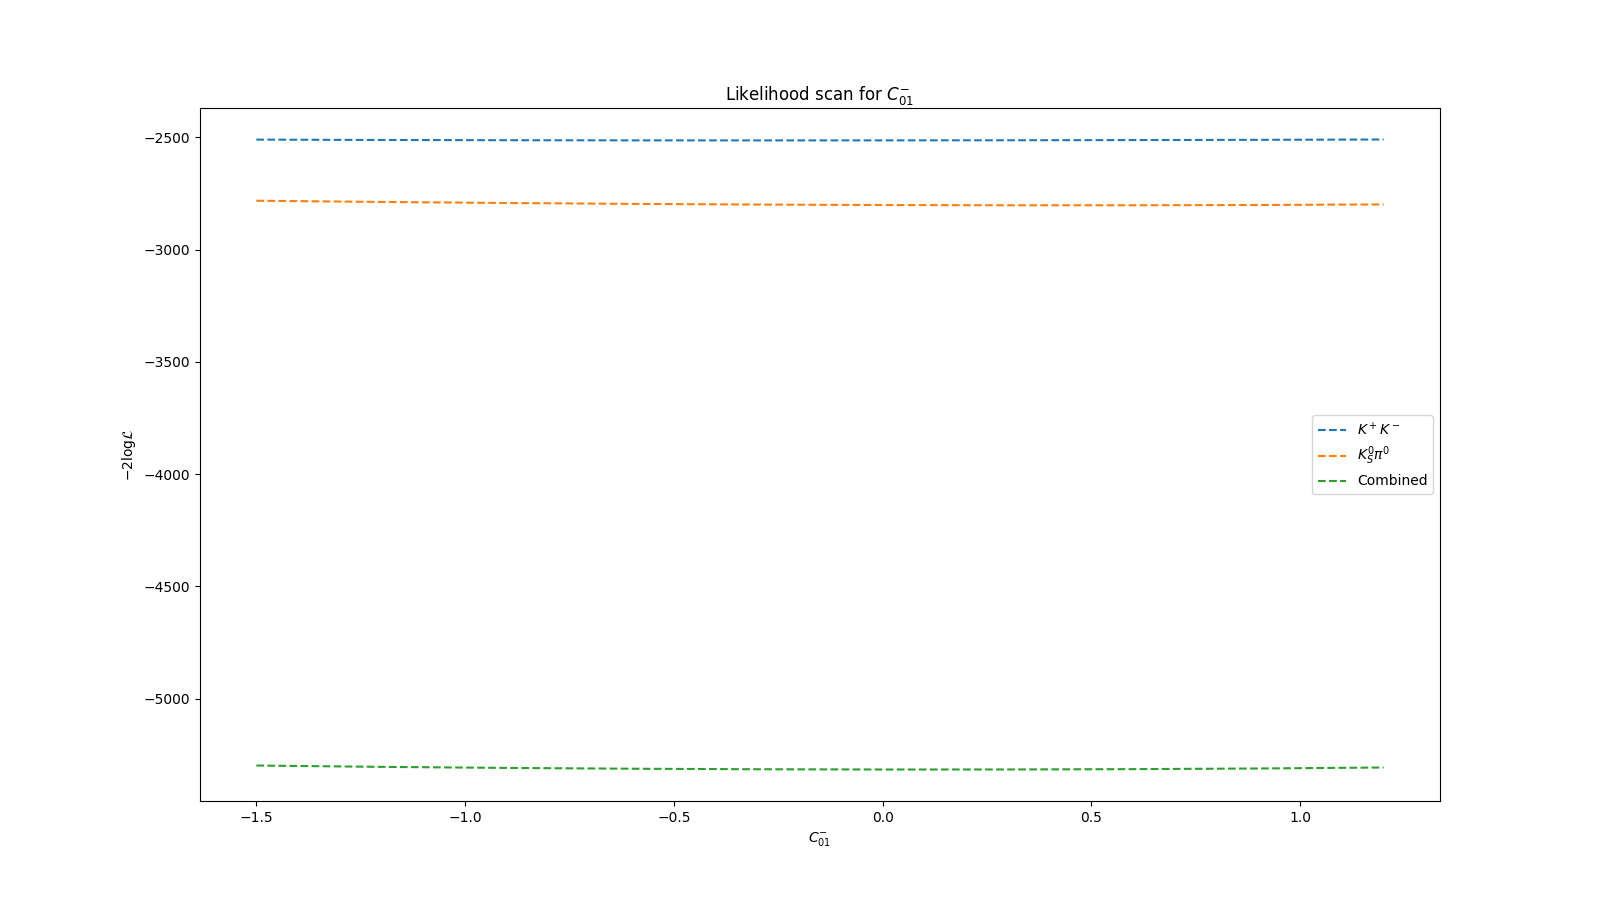
\includegraphics[width=\textwidth]{2020_04_23/figs/M01.png}
    \caption{Likelihood Scan for $C_{01}^{-}$, where the $y$ axis measures the `distance' of the log likelihood at one value of $C_{10}^{-}$.}
    \label{fig:scanCM01}
\end{figure}
\end{frame}

\begin{frame}{Likelihood Scan for $C_{10}^{-}$}
\begin{figure}
    \centering
        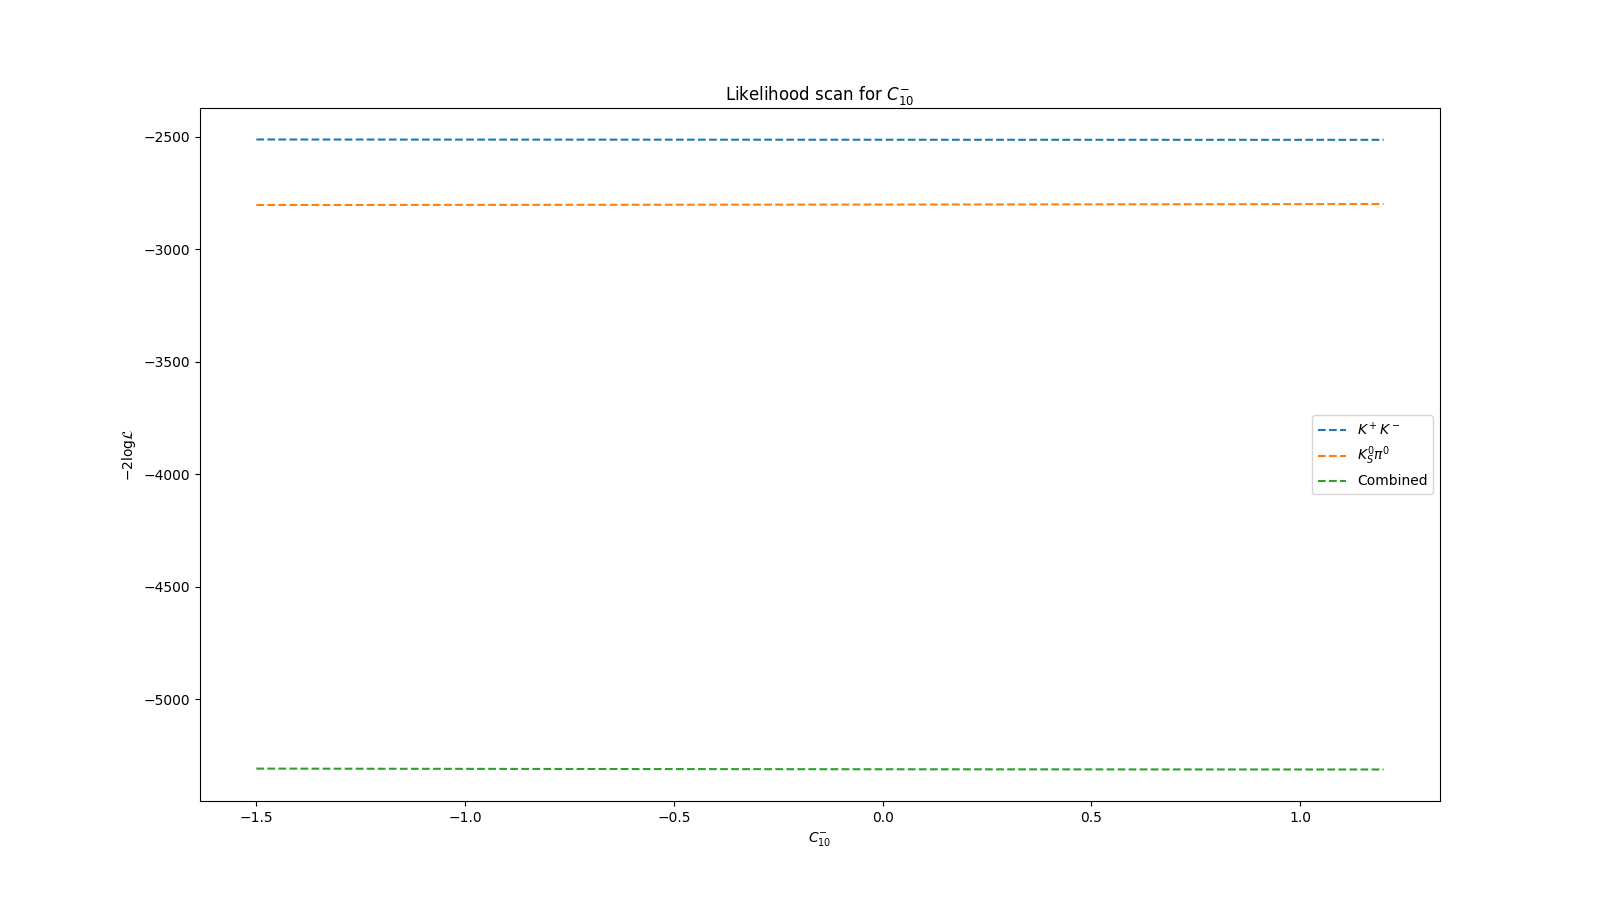
\includegraphics[width=\textwidth]{2020_04_23/figs/M10.png}
    \caption{Likelihood Scan for $C_{10}^{-}$, where the $y$ axis measures the `distance' of the log likelihood at one value of $C_{10}^{-}$.}
    \label{fig:scanCM10}
\end{figure}
\end{frame}

\begin{frame}{Likelihood Scan for $C_{02}^{-}$}
\begin{figure}
    \centering
        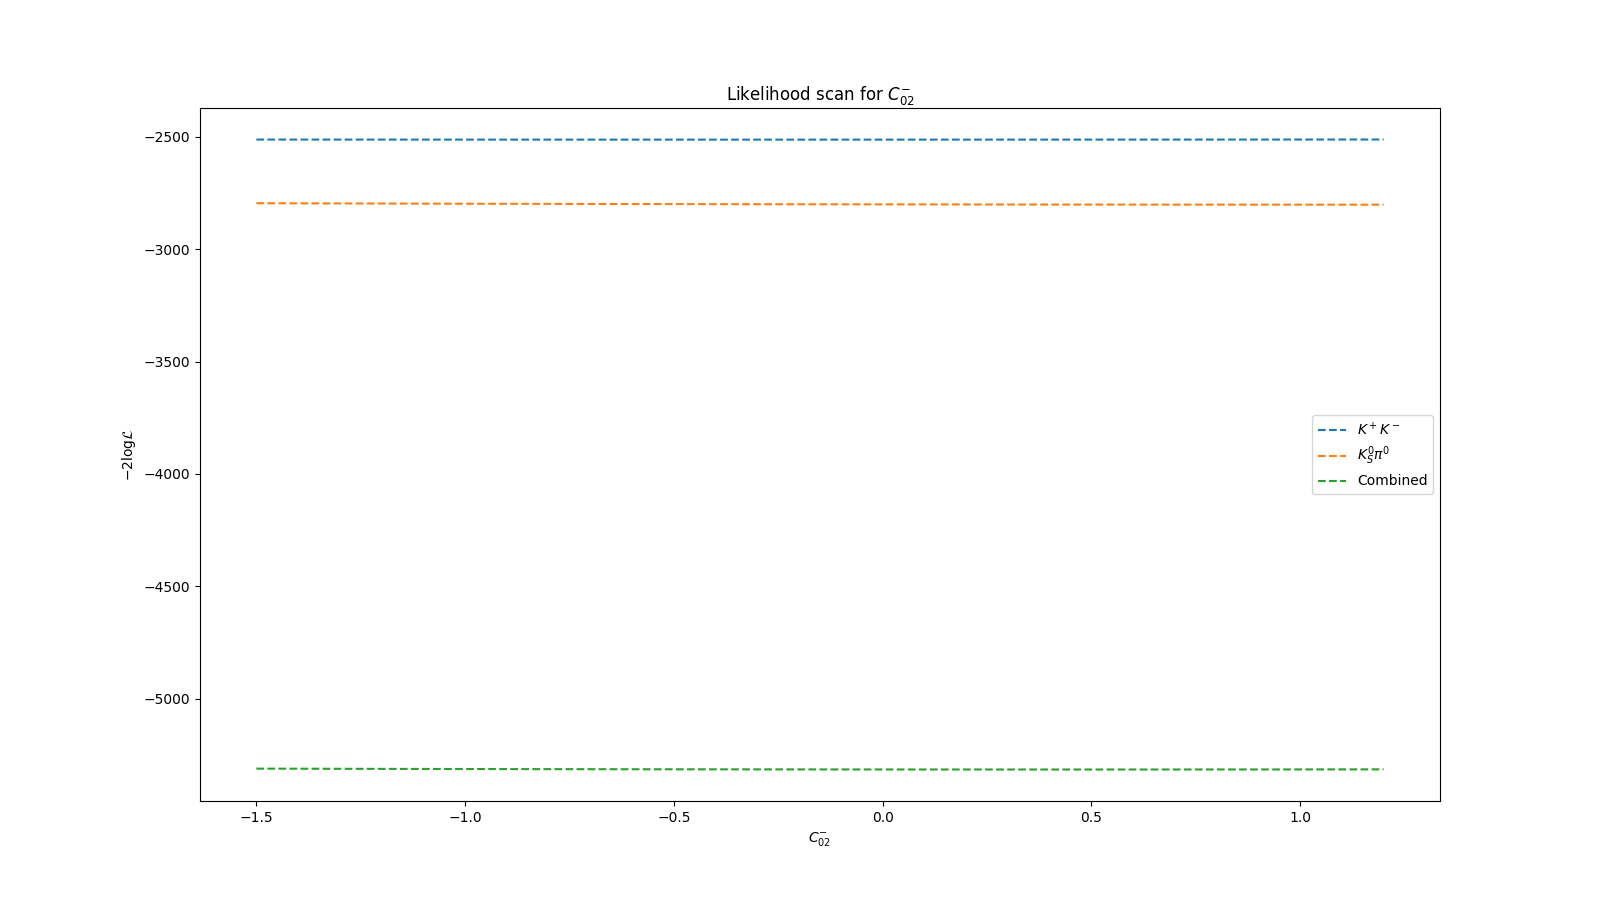
\includegraphics[width=\textwidth]{2020_04_23/figs/M02.png}
    \caption{Likelihood Scan for $C_{02}^{-}$, where the $y$ axis measures the `distance' of the log likelihood at one value of $C_{02}^{-}$.}
    \label{fig:scanCM02}
\end{figure}
\end{frame}

\begin{frame}{Likelihood Scan for $C_{11}^{-}$}
\begin{figure}
    \centering
        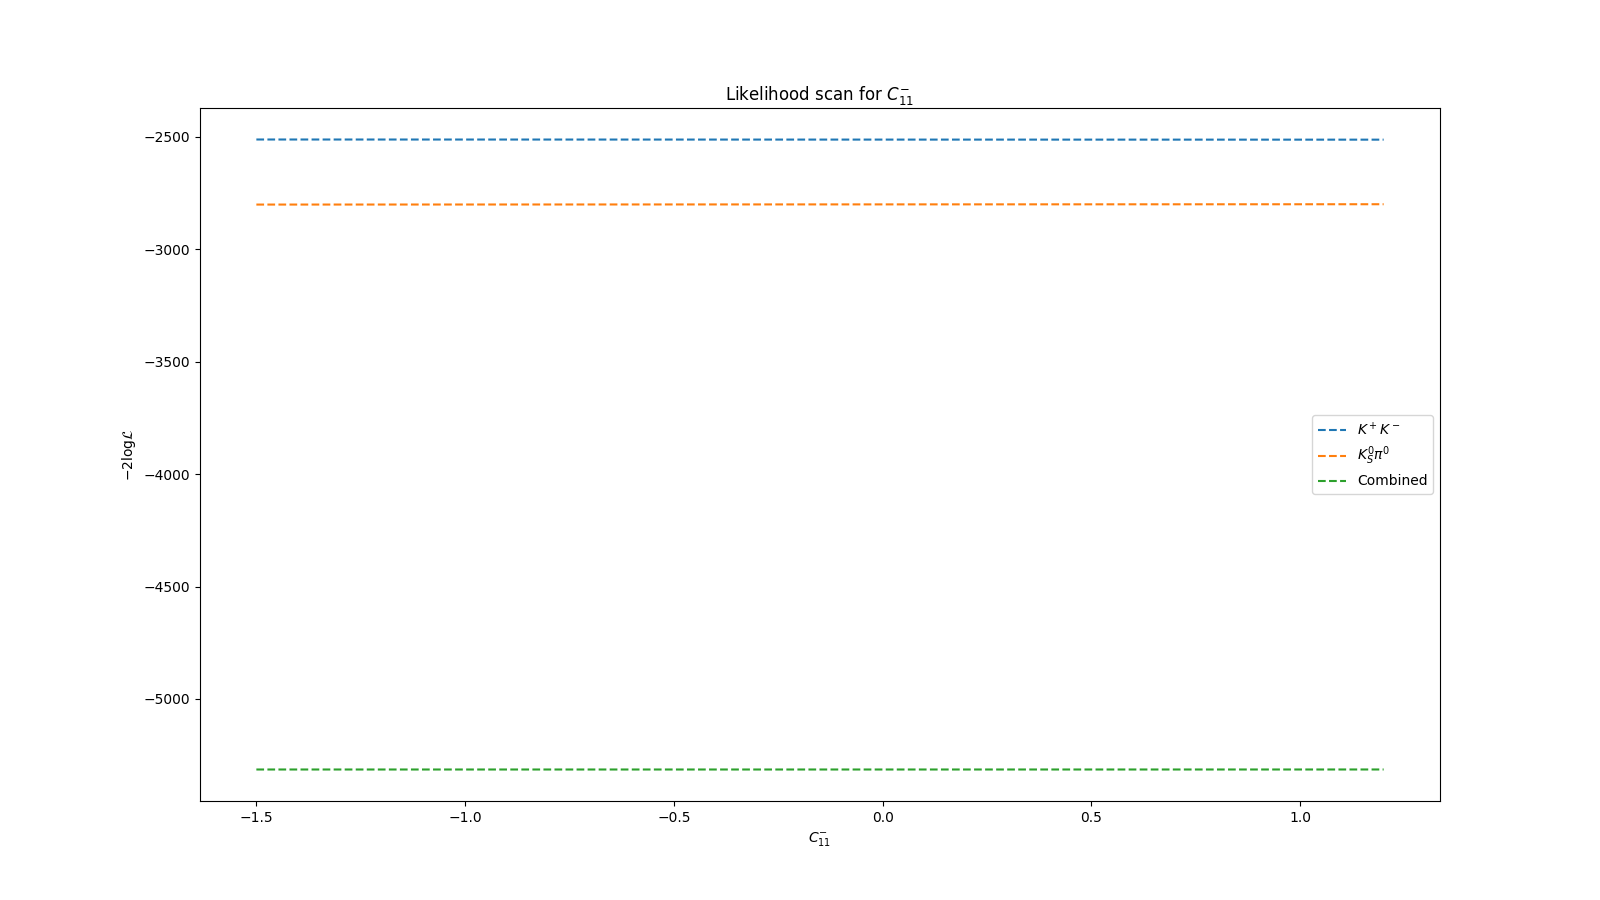
\includegraphics[width=\textwidth]{2020_04_23/figs/M11.png}
    \caption{Likelihood Scan for $C_{11}^{-}$, where the $y$ axis measures the `distance' of the log likelihood at one value of $C_{11}^{-}$.}
    \label{fig:scanCM11}
\end{figure}
\end{frame}


\begin{frame}{Likelihood Scan for $C_{20}^{-}$}
\begin{figure}
    \centering
        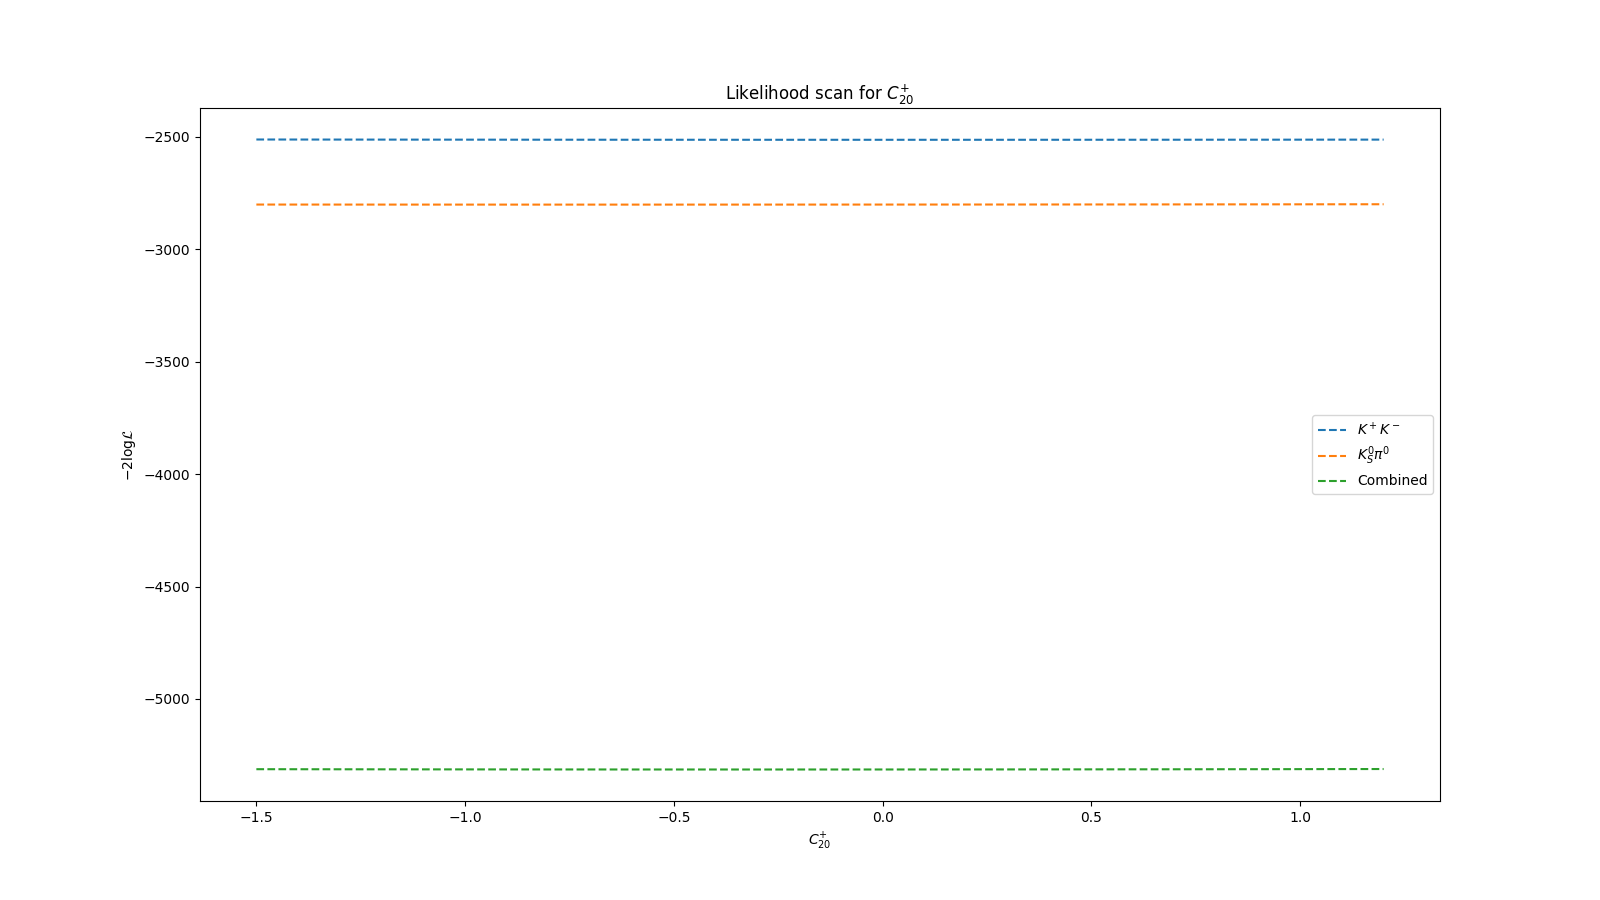
\includegraphics[width=\textwidth]{2020_04_23/figs/P20.png}
    \caption{Likelihood Scan for $C_{20}^{-}$, where the $y$ axis measures the `distance' of the log likelihood at one value of $C_{20}^{-}$.}
    \label{fig:scanCM20}
\end{figure}
\end{frame}



\begin{frame}{Likelihood Scan for $C_{00}^{+}$}
\begin{figure}
    \centering
        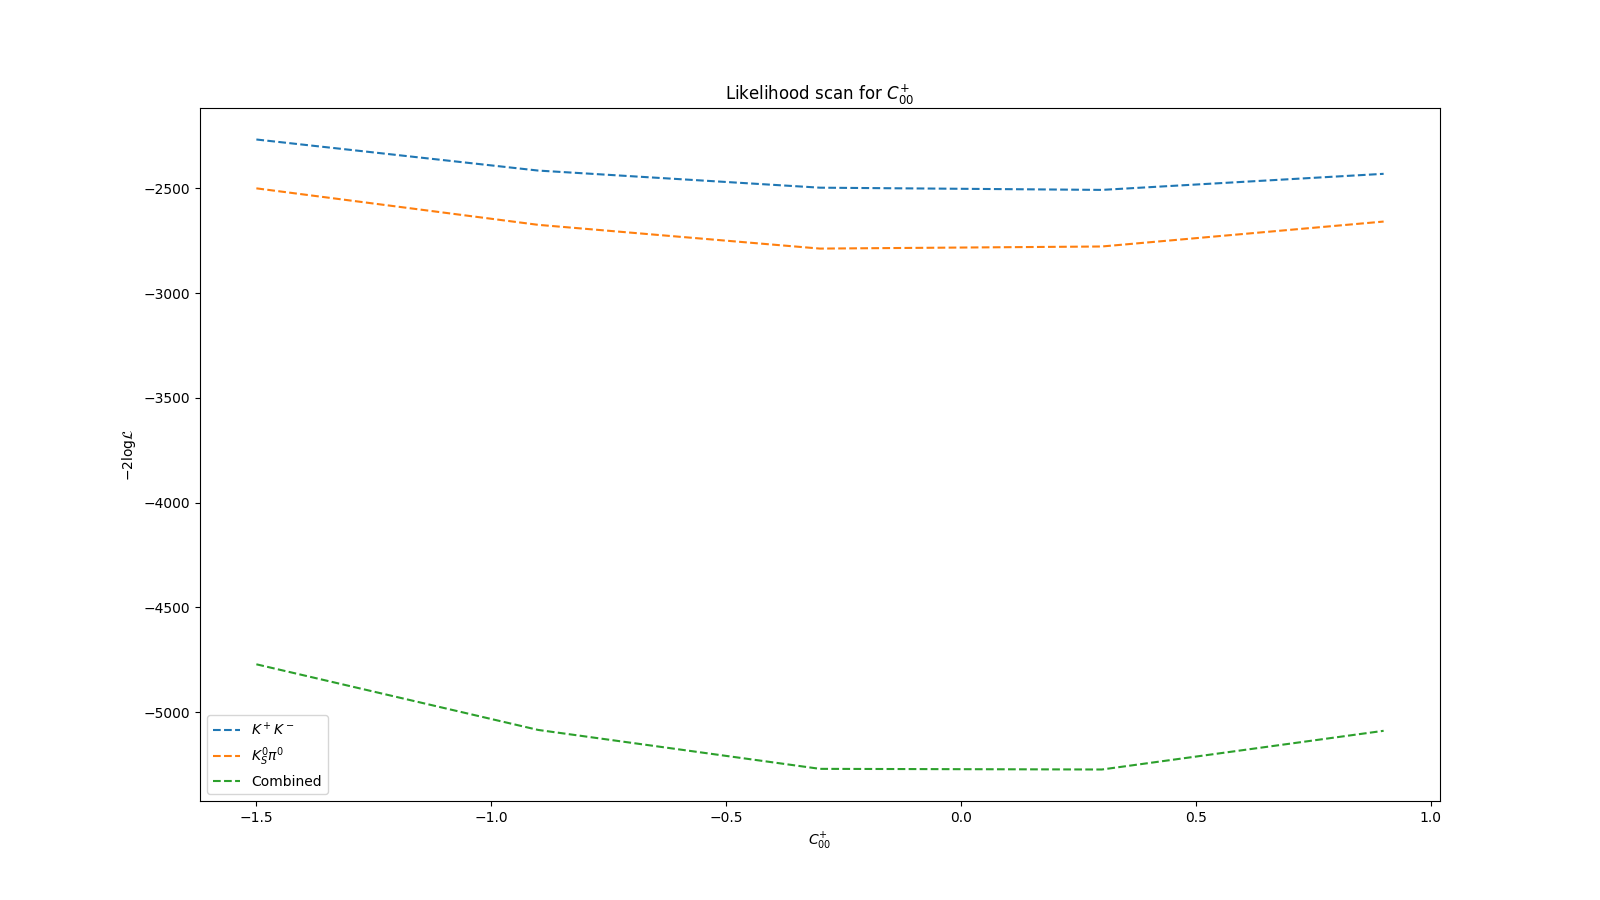
\includegraphics[width=\textwidth]{2020_04_23/figs/P00.png}
    \caption{Likelihood Scan for $C_{00}^{+}$, where the $y$ axis measures the `distance' of the log likelihood at one value of $C_{00}^{+}$.}
    \label{fig:scanCP01}
\end{figure}
\end{frame}

\begin{frame}{Likelihood Scan for $C_{01}^{+}$}
\begin{figure}
    \centering
        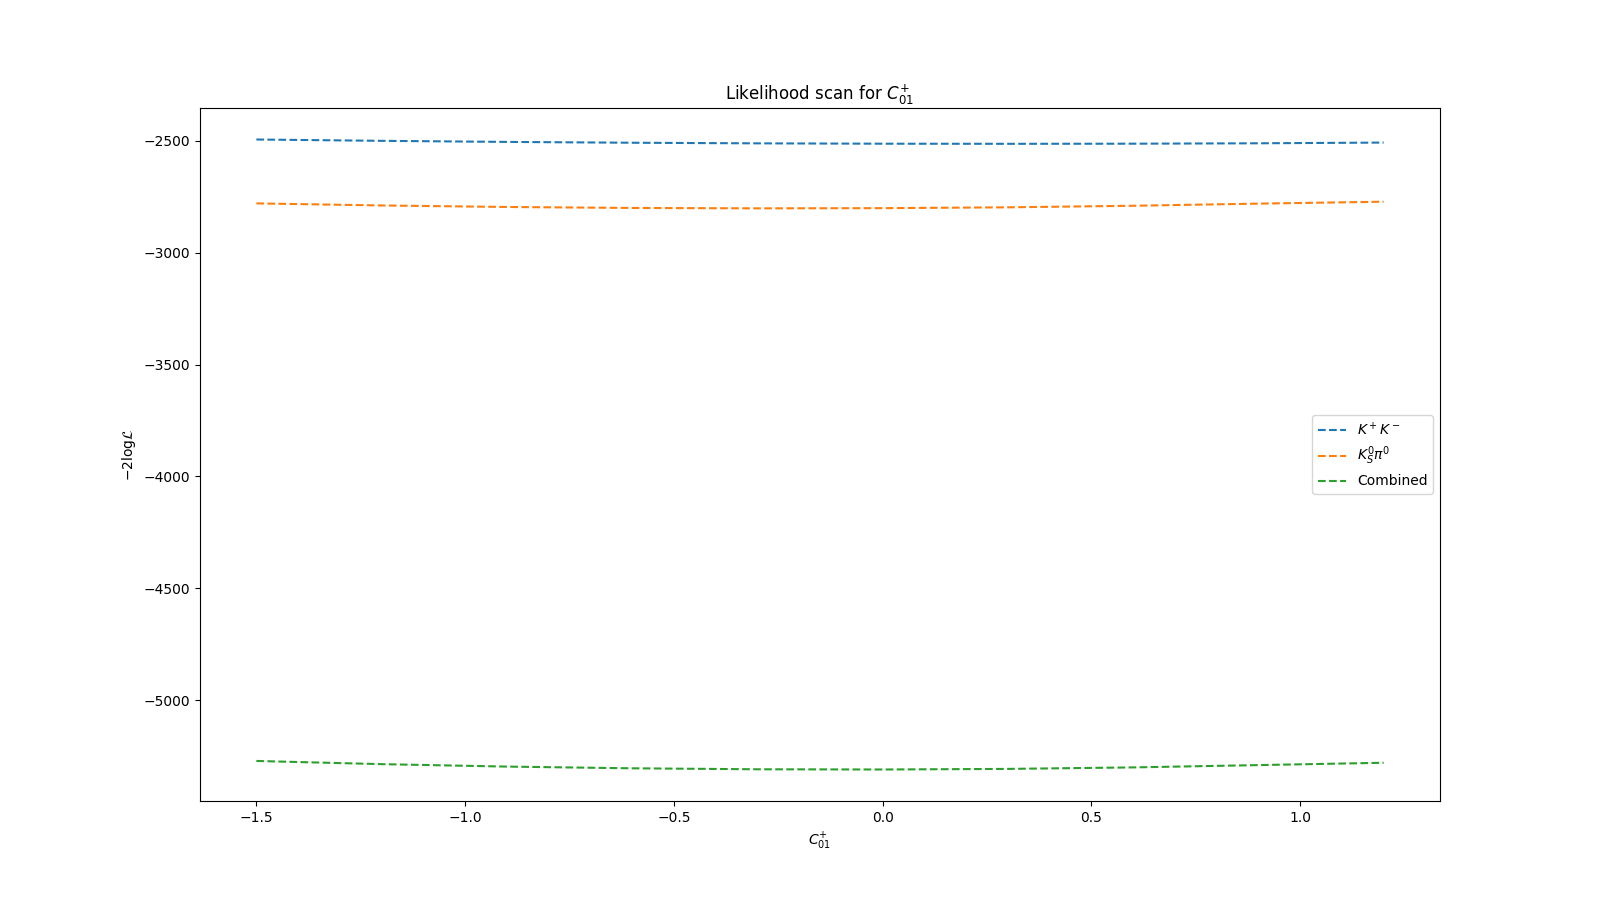
\includegraphics[width=\textwidth]{2020_04_23/figs/P01.png}
    \caption{Likelihood Scan for $C_{01}^{+}$, where the $y$ axis measures the `distance' of the log likelihood at one value of $C_{10}^{+}$.}
    \label{fig:scanCP01}
\end{figure}
\end{frame}

\begin{frame}{Likelihood Scan for $C_{10}^{+}$}
\begin{figure}
    \centering
        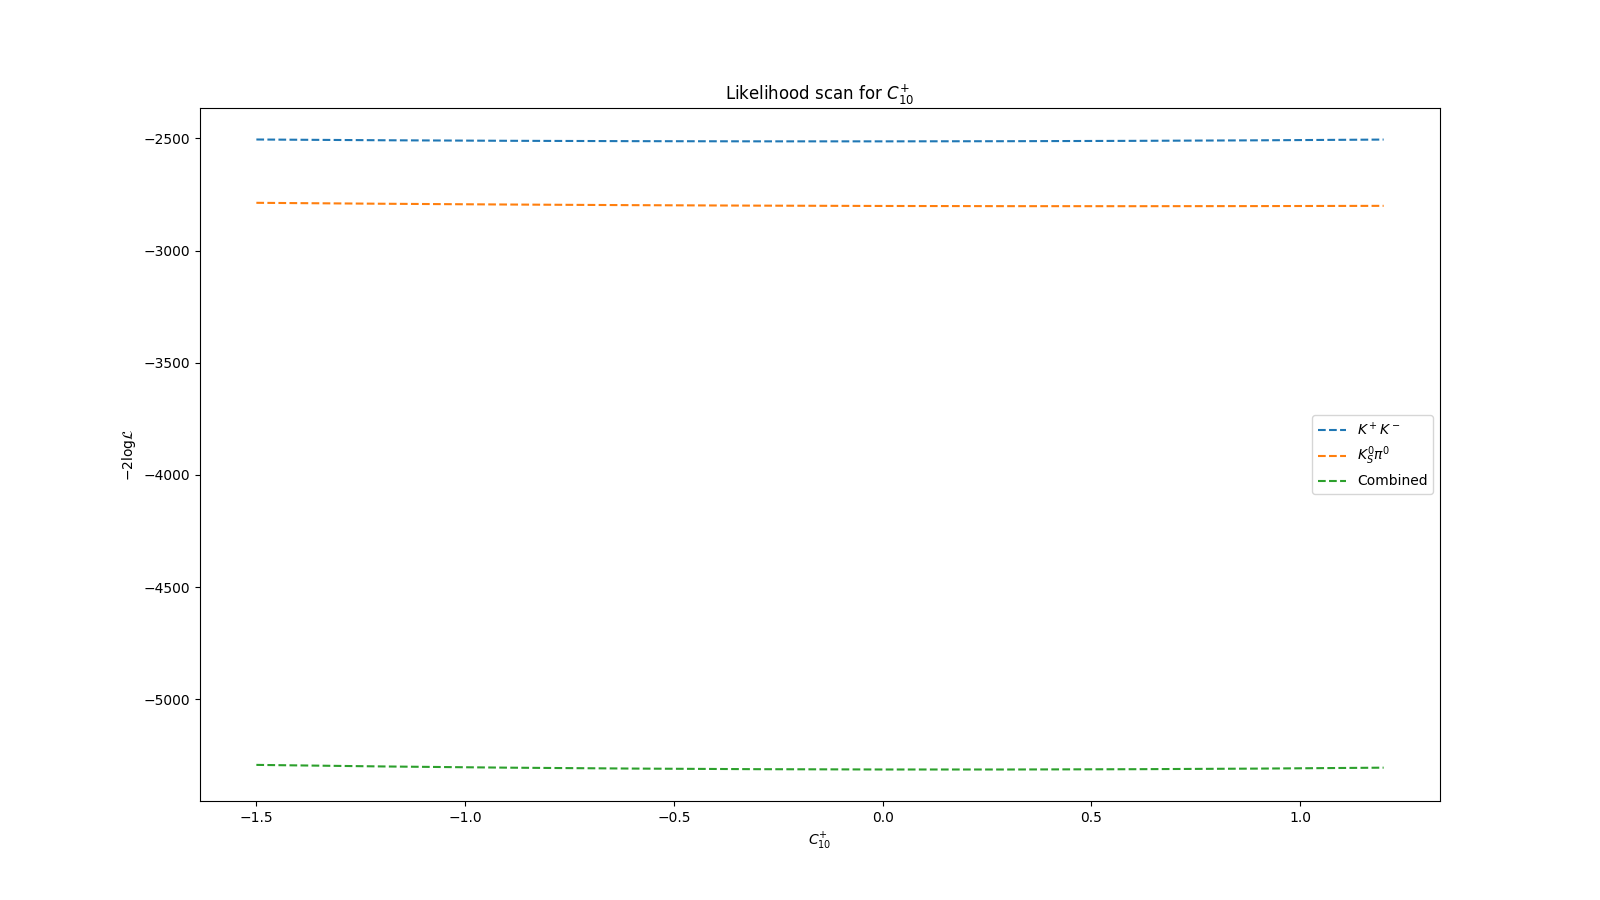
\includegraphics[width=\textwidth]{2020_04_23/figs/P10.png}
    \caption{Likelihood Scan for $C_{10}^{+}$, where the $y$ axis measures the `distance' of the log likelihood at one value of $C_{10}^{+}$.}
    \label{fig:scanCP10}
\end{figure}
\end{frame}

\begin{frame}{Likelihood Scan for $C_{02}^{+}$}
\begin{figure}
    \centering
        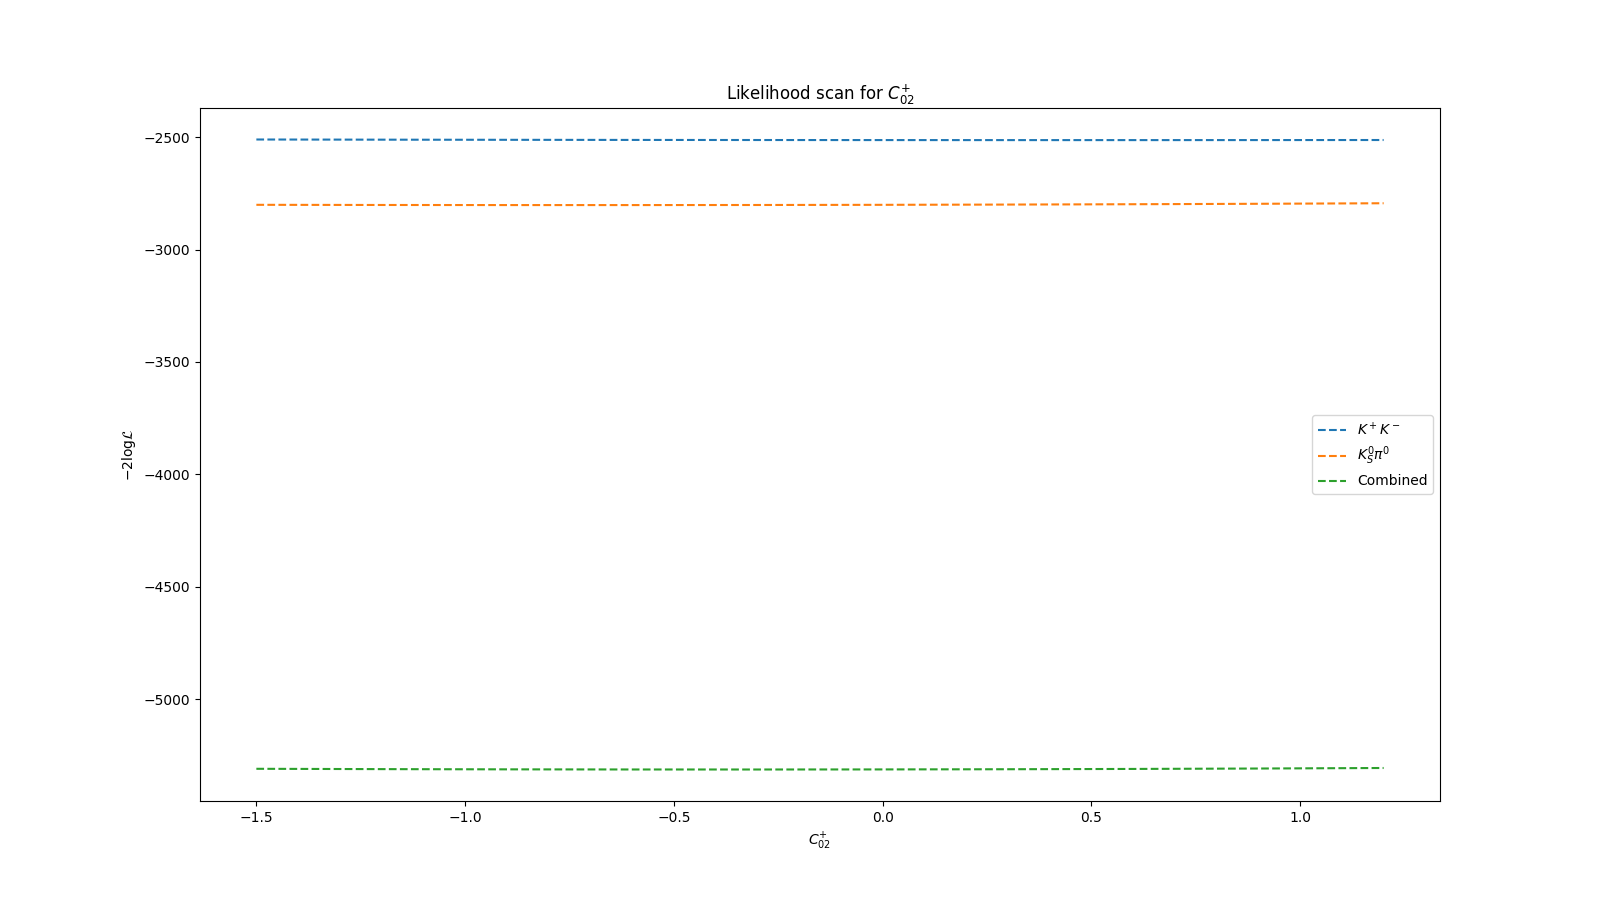
\includegraphics[width=\textwidth]{2020_04_23/figs/P02.png}
    \caption{Likelihood Scan for $C_{02}^{+}$, where the $y$ axis measures the `distance' of the log likelihood at one value of $C_{02}^{+}$.}
    \label{fig:scanCP02}
\end{figure}
\end{frame}

\begin{frame}{Likelihood Scan for $C_{11}^{+}$}
\begin{figure}
    \centering
        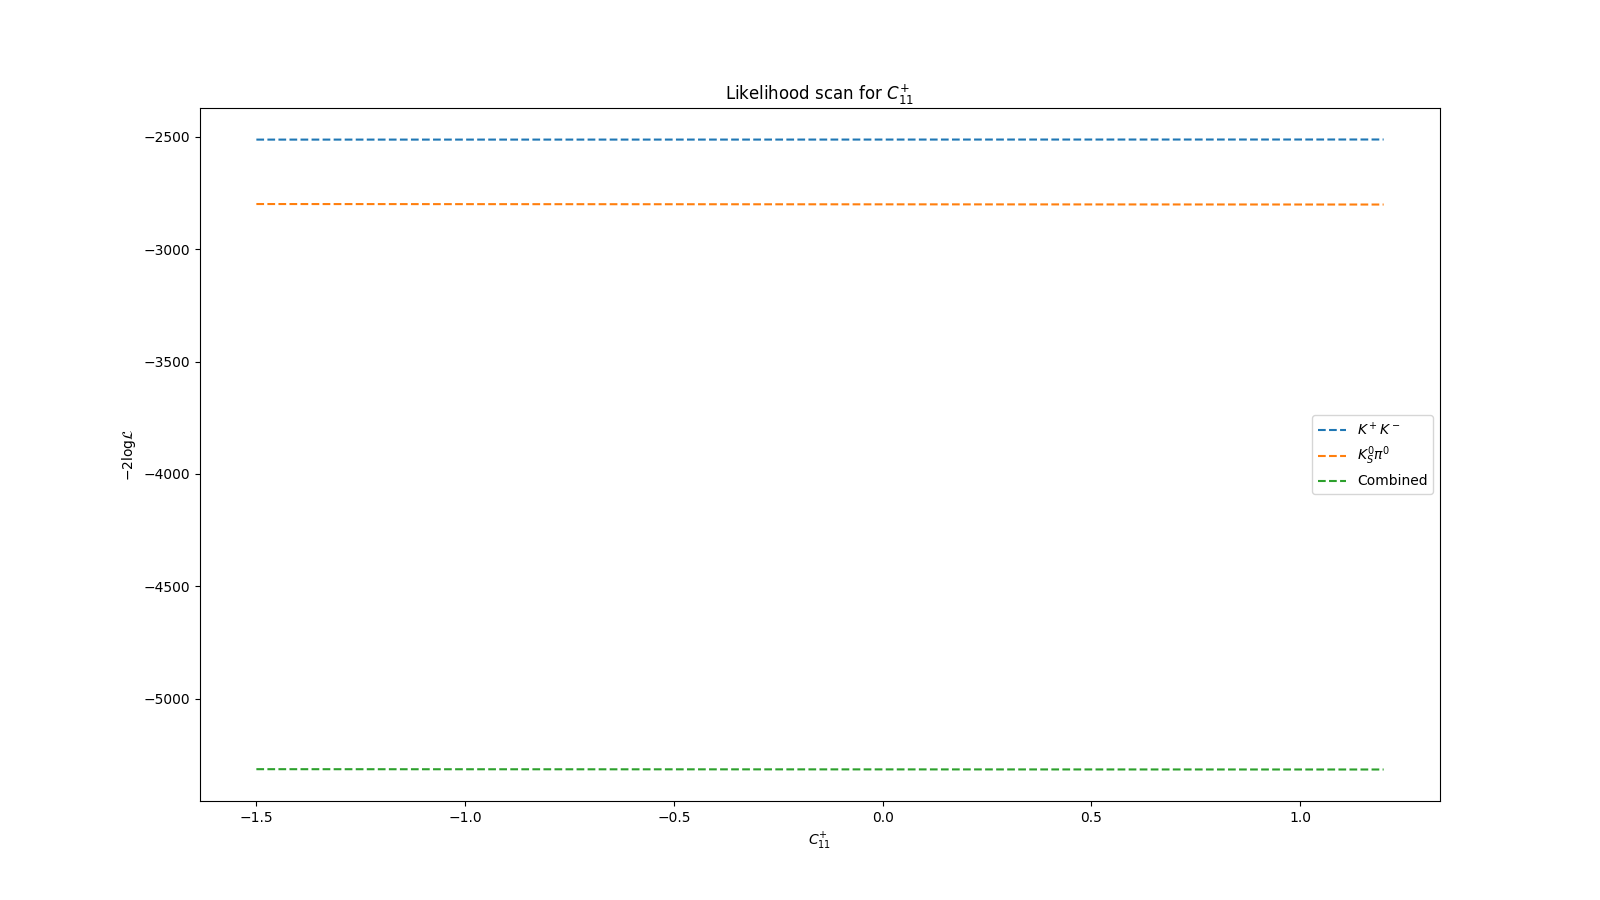
\includegraphics[width=\textwidth]{2020_04_23/figs/P11.png}
    \caption{Likelihood Scan for $C_{11}^{+}$, where the $y$ axis measures the `distance' of the log likelihood at one value of $C_{11}^{+}$.}
    \label{fig:scanCP11}
\end{figure}
\end{frame}


\begin{frame}{Likelihood Scan for $C_{20}^{+}$}
\begin{figure}
    \centering
        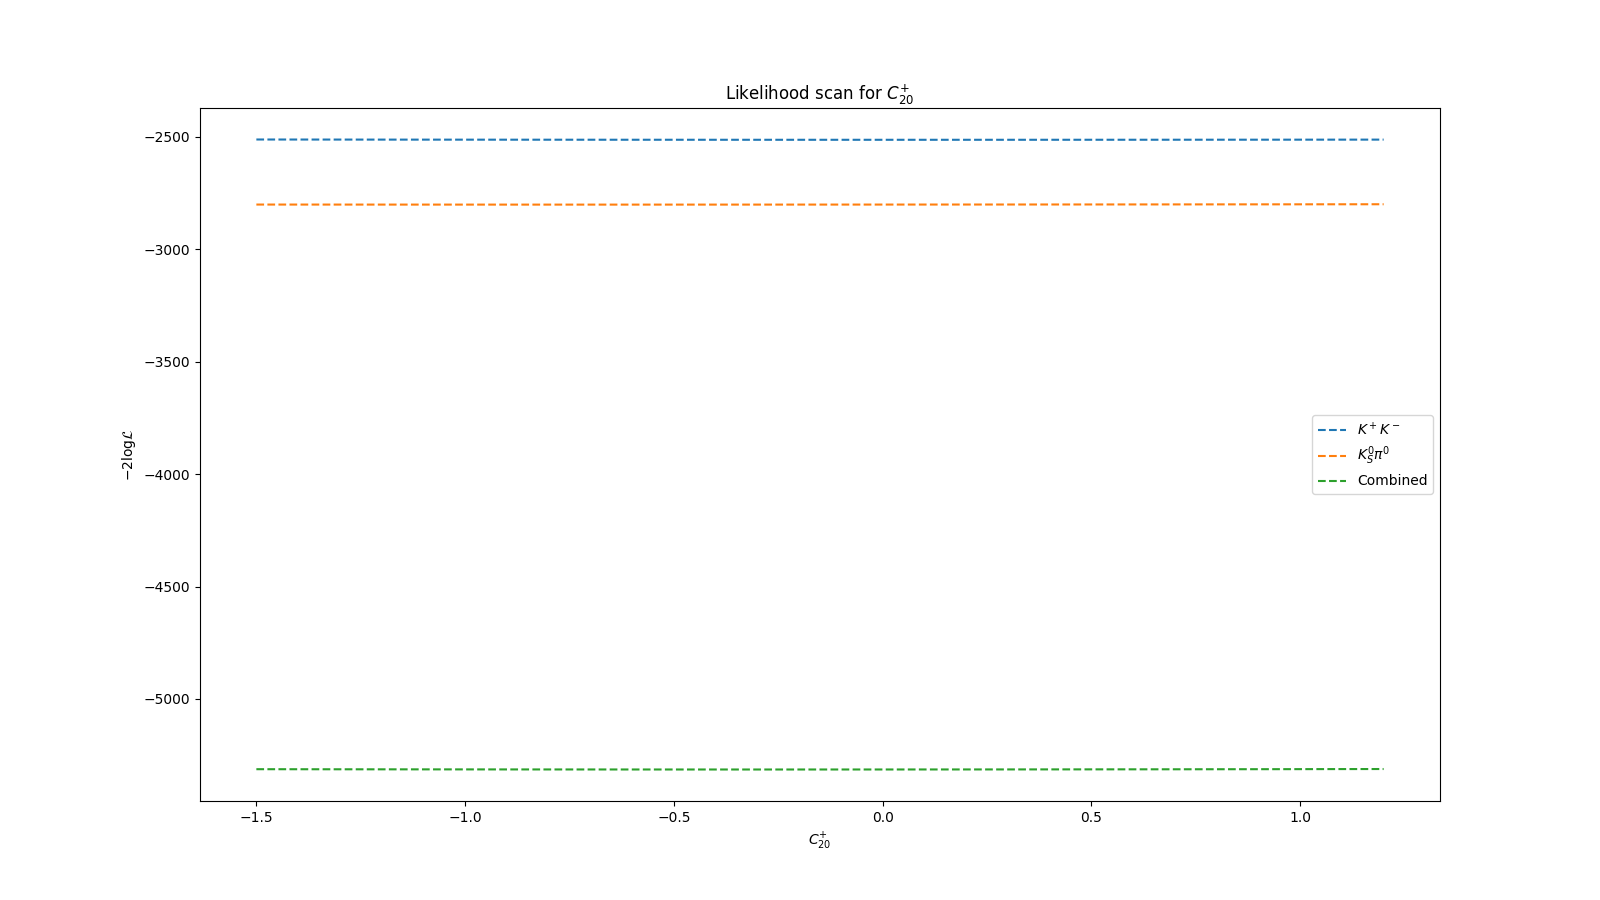
\includegraphics[width=\textwidth]{2020_04_23/figs/P20.png}
    \caption{Likelihood Scan for $C_{20}^{+}$, where the $y$ axis measures the `distance' of the log likelihood at one value of $C_{20}^{+}$.}
    \label{fig:scanCP20}
\end{figure}
\end{frame}



\begin{frame}{Time to perform Likelihood Scan}
we need to calculate 
\begin{equation}
   N_\text{int} = 2 \times N_\text{tag} \times N_\text{param}  = 2 \times N_\text{tag} \times (N_\text{Order} + 1) (N_\text{Order} + 2)
\end{equation}
For $N_\text{Order} = 2$ this is $2 \times 5 \times 3 \times 4 = 120$. Each integral takes $\sim \mathcal{O}(1)m$, i.e. for all of our tags we would expect up to $\sim 30m - 2h$ per value - i.e. it would take anywhere from $5h - 20h$ to make a full plot for every parameter. If we run each job on a $\mathcal{O}(10)$ core computer, we can hope to reduce this time by a factor $10$, i.e. instead of $\mathcal{O}(10)h$ we could do it in $\mathcal{O}(1)$h.
When testing we can reduce this time by a few factors - e.g. only using 2-3 tags and with only 2-3 different values for one parameter would only take $2 \times 3 \times 1 \times \mathcal{O}(1) \sim \mathcal{O}(5)$ minutes. 
\end{frame}
\begin{frame}{From Appendix of the note}
We wish to minimise the function
\begin{equation}
    -2\log\mathcal{L}_\text{comb} \equiv \sum_\text{tag} \left(-2 \log \mathcal{L}_\text{tag}\right) \label{eqn:combLL},
\end{equation}
where we construct a log-likelihood for each tag.

To perform this sum in \texttt{AmpGen} we have two options
\begin{enumerate}
    \item Make a \texttt{std::vector} of $-2\log\mathcal{L}_\text{tag}$ objects, \texttt{CorrelatedLL}, \texttt{\{CorrLL\_KK, CorrLL\_Kppim,...\}}, and calculate (\ref{eqn:combLL}),
    \item Make the object that calculates (\ref{eqn:combLL}) with \texttt{std::vector} versions of the input to \texttt{CorrelatedLL},
\end{enumerate}
in the first case, we found that \texttt{AmpGen} crashes when initialising the combined log-likelihood - this is likely an issue with memory management in the \texttt{C++} code implementing this combined object. 
\end{frame}
\begin{frame}


The second solution should avoid this by using only one instance of \texttt{MPS}, we build an object with the following inputs
\begin{enumerate}
    \item Four \texttt{std::vector}'s of \texttt{EventList}'s, \texttt{\{ SigData\_KK, SigData\_Kppim, ... \}} and \texttt{\{ TagData\_KK, TagData\_Kppim, ... \}} for the ``Data'' events (that we wish to fit) for both ``Signal'' (\texttt{Sig}) and ``tag'' (\texttt{Tag}) and \texttt{\{ SigInt\_KK, SigInt\_Kppim, ... \}} and \texttt{\{ TagInt\_KK, TagInt\_Kppim, ... \}} for the ``Integration'' events - which (for the moment) is needed as an input to normalise the correlated amplitude for each tag.
    \item Two \texttt{std::vector}'s of \texttt{EventType}'s, \texttt{\{SigType\_KK, SigType\_Kppim, ...\}} and \texttt{\{TagType\_KK, TagType\_Kppim, ...\}},
    \item A single \texttt{MinuitParameterSet} object that contains all of the information for every amplitude we intend to build.
\end{enumerate}
\end{frame}
\begin{frame}
We then build the combined log-likelihood in a single object by evaluating the sum
\begin{equation}
    \begin{split}
    -2\log\mathcal{L}_\text{comb} &=-2 \sum_\text{tag} \sum_{\z_1,\z_2 \in \textbf{Z}^\text{tag}_1, \textbf{Z}^\text{tag}_2} \log\left|\Psi_\text{tag}(\z_1, \z_2)\right|^2, \\ 
    \mathbf{Z}^\text{tag}_1, \mathbf{Z}^\text{tag}_2 &= \texttt{SigData\_tag}, \texttt{TagData\_tag},\label{eqn:fullCombLL}
    \end{split}
\end{equation}
now any change to \texttt{MPS} will cause \texttt{AmpGen} to recalculate the sum (\ref{eqn:fullCombLL}) , and any changes to the $\Psi_\text{tag}$ are also reevaluated (including changes to the normalisation of $\Psi_\text{tag}$).
\end{frame}

\newcommand{\LLScan}[1]{

\begin{frame}{Likelihood scan for $C_{#1}$}
\includegraphics[width=\textwidth]{2020_04_28/figs/#1_Norm.png}
NB The straight line is a plotting artefact from \texttt{pyplot}
\end{frame}
}


\newcommand{\pull}[2]{
\begin{frame}{Pull distribution for #2 }
\includegraphics[width=\textwidth]{2020_04_28/figs/#1.png}
\end{frame}

}

\newcommand{\pullDist}[3]{
\begin{frame}{Pull distribution for $C_{#1}$ with the #3 tag}
\includegraphics[width=\textwidth]{2020_04_28/figs/pulls/#2_#1.png}
\end{frame}

}
\newcommand{\diffDist}[3]{
\begin{frame}{Pull distribution for $C_{#1}$ with the #3 tag}
\includegraphics[width=\textwidth]{2020_04_28/figs/diffs/#2_#1.png}
\end{frame}

}


\newcommand{\dists}[3]{
\begin{frame}{$C_{#1}$ with the #3}
\begin{columns}
\begin{column}{0.5\textwidth}
\includegraphics[width=\textwidth]{2020_04_28/figs/diffs/#2_#1.png}
\end{column}
\begin{column}{0.5\textwidth}
\includegraphics[width=\textwidth]{2020_04_28/figs/pulls/#2_#1.png}
\end{column}
\end{columns}

Left : Distribution of $C_{#1}^\text{Fit} - C_{#1}^\text{True}$,

right : $(C_{#1}^\text{Fit} - C_{#1}^\text{True})/\sigma C_{#1}^\text{Fit}$
\end{frame}

}

\newcommand{\alldists}[2]{
\dists{00}{#1}{#2}
\dists{01}{#1}{#2}
\dists{10}{#1}{#2}
\dists{02}{#1}{#2}
\dists{11}{#1}{#2}
\dists{02}{#1}{#2}
}

\begin{frame}{Overview}
    \begin{itemize}
        \item After considering physical constraints on $\dd$, we change our proposed ``CP-polynomial'' to an ``anti-symmetric'' polynomial
        \item Widen the range for the likelihood scan for each component
        \item Perform a pull study for the ``anti-symmetric'' polynomial
    \end{itemize}
\end{frame}
\begin{frame}
    Given that 
    \begin{equation}
        \dd(\MM,\MP) = -\dd(\MP,\MM),
    \end{equation}
    and that the model $\dd$ ($\dd^\text{model}$) satisfies this, any correction to $\dd^\text{model}$ ($f(\MM,\MP)$) must also satisfy (1), i.e. the so-called ``CP-Negative'' polynomial, which we will rename to the anti-symmetric polynomial since the function is anti-symmetric along the line $\MM=\MP$, using the parameterisation $w_\pm = (z_+ \pm z_-)/2$ where $z_\pm$ is a re-scaled $m^2_\pm$ such that $z_\pm \in (-1,1)$,
    \begin{equation}
        f(w_-,w_+) = \sum_{i=0}^{N_\text{Order}} \sum_{j=0}^{N_\text{Order} - i} C_{ij} P_{i}(w_+) P_{2j+1}(w_-)
    \end{equation}
\end{frame}

\begin{frame}{$\dd$ plot}
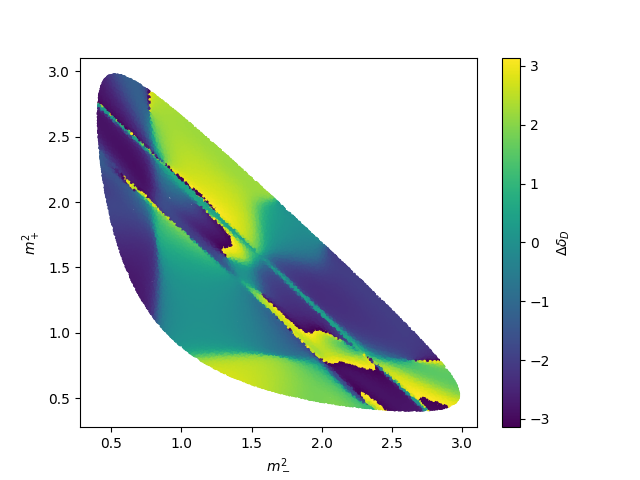
\includegraphics[width=\textwidth]{2020_04_28/figs/dd.png}
\end{frame}
\LLScan{00}
\LLScan{01}
\LLScan{10}
\LLScan{02}
\LLScan{11}
\LLScan{20}

\begin{frame}{Pull Studies}
\begin{enumerate}
    \item Generate $N=10000$ sample from the Belle-BaBar 2018 model
    \item Tags are \KK, \Kspiz, \Kppim, \Kmpip, \Kspipi and the combined tag
    \item \Kppim and \Kmpip tags are modified such that the wrong sign couplings are $-0.0537\pm0.032i$ (back of envelope calculation)
    \item Fit with $N_\text{Order}=2$ polynomial
\end{enumerate}{}
\end{frame}

\pull{KK}{\KK}
\pull{Kmpip}{\Kmpip}
\pull{Kppim}{\Kppim}
\pull{Kspi0}{\Kspiz}
\pull{Kspipi}{\Kspipi}
\pull{Comb}{Combined tags}



\newcommand{\pull}[3]{
\begin{frame}{Pull distribution for #3}
\includegraphics[width=\textwidth]{2020_05_14/figs/antiSym_#1/antiSym_#1/4/pulls/#2.png}
\end{frame}

}


\newcommand{\pulls}[1]{
    \pull{#1}{Comb}{Combined Tag}
    \pull{#1}{KK}{$\KK$ tag}
    \pull{#1}{Kspi0}{$\Kspiz$ tag}
    \pull{#1}{Kppim}{$\Kppim$ tag}
    \pull{#1}{Kmpip}{$\Kmpip$ tag} 
    \pull{#1}{Kspipi}{$\Kspipi$ tag}
}


\newcommand{\projod}[5]{
    \begin{frame}{Projection for #5}


        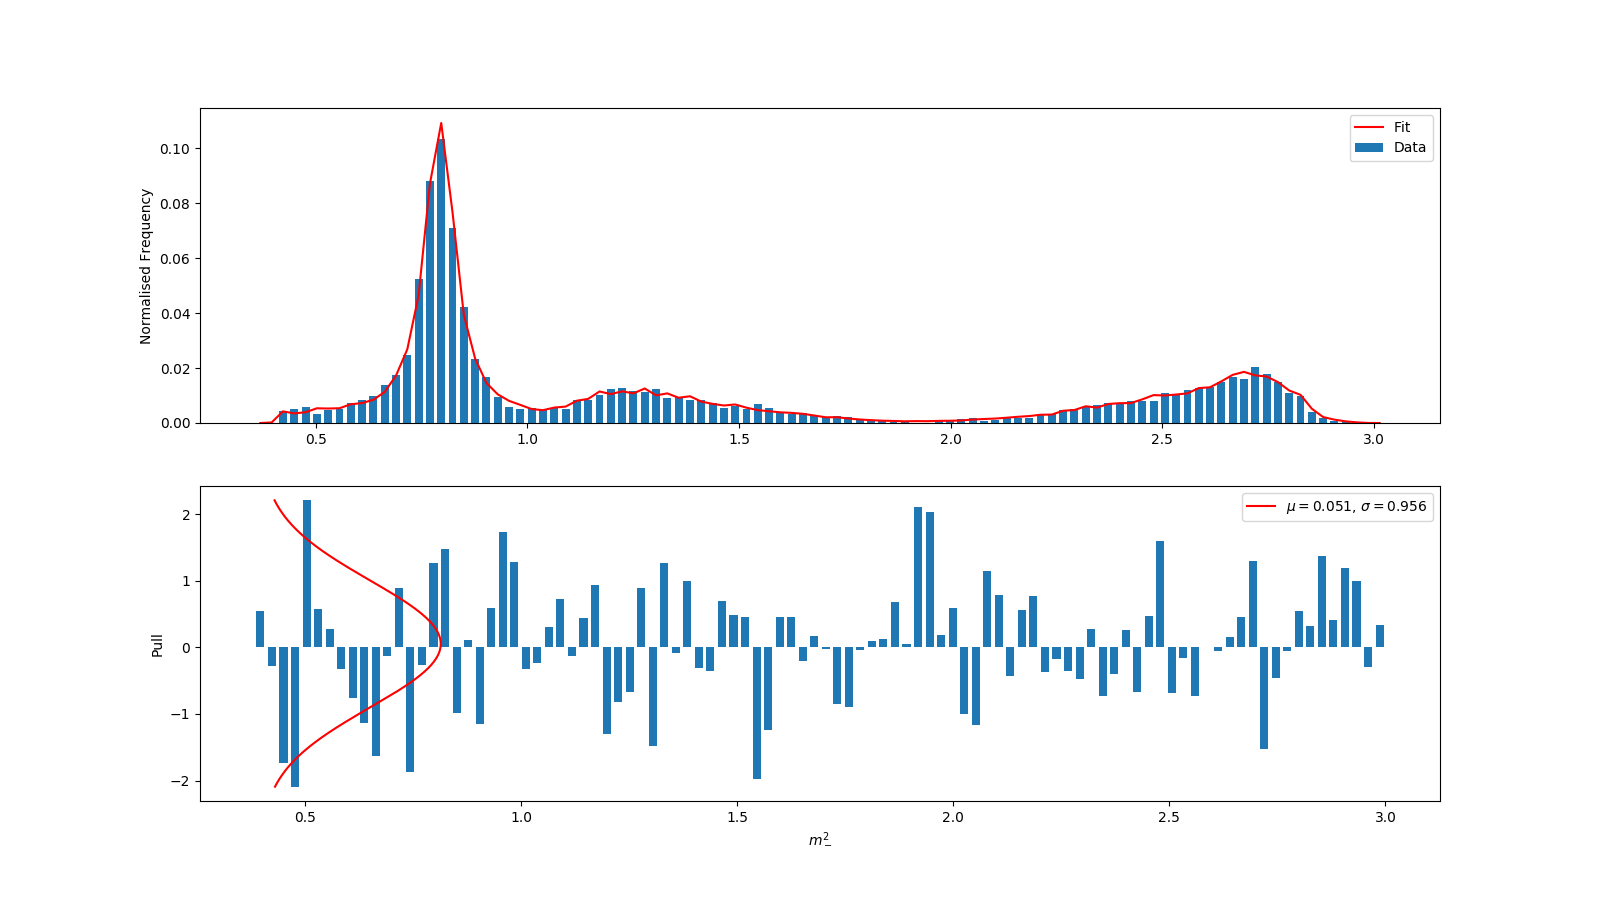
\includegraphics[width=\textwidth]{2020_05_14/figs/antiSym_#1/antiSym_#1/proj/#2/#3/#4/s01.png}

    \end{frame}

    \begin{frame}{Projection for #5}
            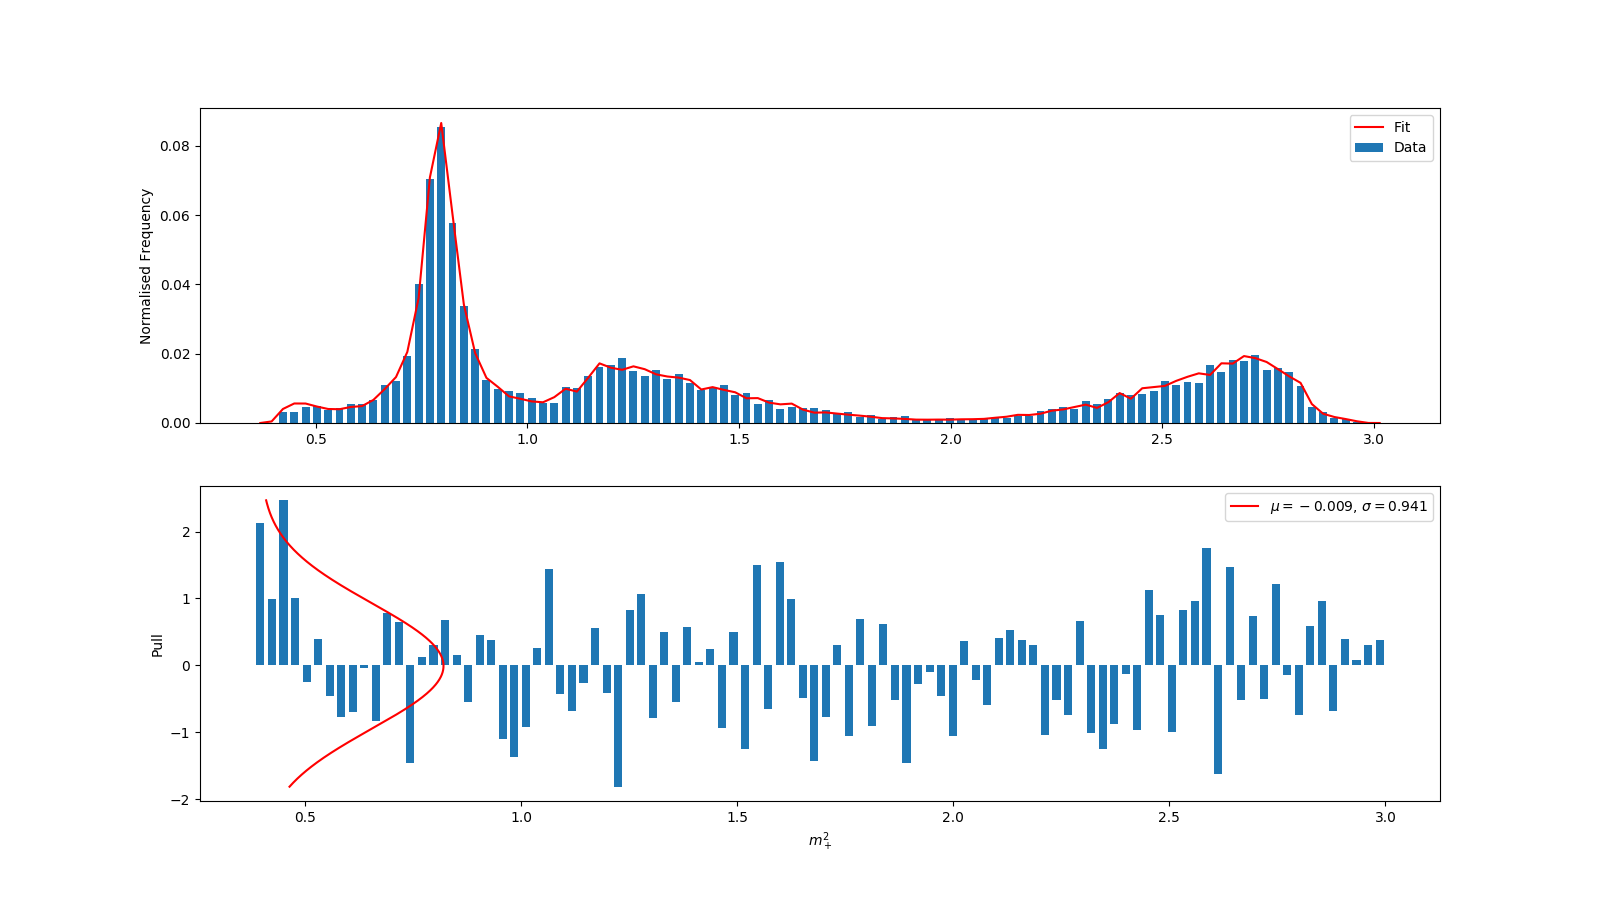
\includegraphics[width=\textwidth]{2020_05_14/figs/antiSym_#1/antiSym_#1/proj/#2/#3/#4/s02.png}

   

    \end{frame}
}

\newcommand{\projtd}[5]{
    \begin{frame}{Projection for #5}


                \includegraphics[width=\textwidth]{2020_05_14/figs/antiSym_#1/antiSym_#1/proj/#2/#3/#4_s01_vs_s02.png}

    \end{frame}
    \begin{frame}{Projection for #5}

                \includegraphics[width=\textwidth]{2020_05_14/figs/antiSym_#1/antiSym_#1/proj/#2/#3/#4_s01_vs_s02_pull.png}


    \end{frame}

}

\newcommand{\allprojod}[3]{
    \projod{#1}{#2}{#3}{KK}{s01}
    \projod{#1}{#2}{#3}{Kspi0}{s01}
    \projod{#1}{#2}{#3}{Kppim}{s01}
    \projod{#1}{#2}{#3}{Kmpip}{s01}
    \projod{#1}{#2}{#3}{Kspipi}{s01}

}

\pulls{chebyshev}
\pulls{simple}
\projod{simple}{136}{0}{KK}{s01}
\projtd{simple}{136}{0}{KK}{s01}

\end{document}